% Options for packages loaded elsewhere
\PassOptionsToPackage{unicode}{hyperref}
\PassOptionsToPackage{hyphens}{url}
%
\documentclass[
]{book}
\usepackage{amsmath,amssymb}
\usepackage{lmodern}
\usepackage{iftex}
\ifPDFTeX
  \usepackage[T1]{fontenc}
  \usepackage[utf8]{inputenc}
  \usepackage{textcomp} % provide euro and other symbols
\else % if luatex or xetex
  \usepackage{unicode-math}
  \defaultfontfeatures{Scale=MatchLowercase}
  \defaultfontfeatures[\rmfamily]{Ligatures=TeX,Scale=1}
\fi
% Use upquote if available, for straight quotes in verbatim environments
\IfFileExists{upquote.sty}{\usepackage{upquote}}{}
\IfFileExists{microtype.sty}{% use microtype if available
  \usepackage[]{microtype}
  \UseMicrotypeSet[protrusion]{basicmath} % disable protrusion for tt fonts
}{}
\makeatletter
\@ifundefined{KOMAClassName}{% if non-KOMA class
  \IfFileExists{parskip.sty}{%
    \usepackage{parskip}
  }{% else
    \setlength{\parindent}{0pt}
    \setlength{\parskip}{6pt plus 2pt minus 1pt}}
}{% if KOMA class
  \KOMAoptions{parskip=half}}
\makeatother
\usepackage{xcolor}
\usepackage{color}
\usepackage{fancyvrb}
\newcommand{\VerbBar}{|}
\newcommand{\VERB}{\Verb[commandchars=\\\{\}]}
\DefineVerbatimEnvironment{Highlighting}{Verbatim}{commandchars=\\\{\}}
% Add ',fontsize=\small' for more characters per line
\usepackage{framed}
\definecolor{shadecolor}{RGB}{248,248,248}
\newenvironment{Shaded}{\begin{snugshade}}{\end{snugshade}}
\newcommand{\AlertTok}[1]{\textcolor[rgb]{0.94,0.16,0.16}{#1}}
\newcommand{\AnnotationTok}[1]{\textcolor[rgb]{0.56,0.35,0.01}{\textbf{\textit{#1}}}}
\newcommand{\AttributeTok}[1]{\textcolor[rgb]{0.77,0.63,0.00}{#1}}
\newcommand{\BaseNTok}[1]{\textcolor[rgb]{0.00,0.00,0.81}{#1}}
\newcommand{\BuiltInTok}[1]{#1}
\newcommand{\CharTok}[1]{\textcolor[rgb]{0.31,0.60,0.02}{#1}}
\newcommand{\CommentTok}[1]{\textcolor[rgb]{0.56,0.35,0.01}{\textit{#1}}}
\newcommand{\CommentVarTok}[1]{\textcolor[rgb]{0.56,0.35,0.01}{\textbf{\textit{#1}}}}
\newcommand{\ConstantTok}[1]{\textcolor[rgb]{0.00,0.00,0.00}{#1}}
\newcommand{\ControlFlowTok}[1]{\textcolor[rgb]{0.13,0.29,0.53}{\textbf{#1}}}
\newcommand{\DataTypeTok}[1]{\textcolor[rgb]{0.13,0.29,0.53}{#1}}
\newcommand{\DecValTok}[1]{\textcolor[rgb]{0.00,0.00,0.81}{#1}}
\newcommand{\DocumentationTok}[1]{\textcolor[rgb]{0.56,0.35,0.01}{\textbf{\textit{#1}}}}
\newcommand{\ErrorTok}[1]{\textcolor[rgb]{0.64,0.00,0.00}{\textbf{#1}}}
\newcommand{\ExtensionTok}[1]{#1}
\newcommand{\FloatTok}[1]{\textcolor[rgb]{0.00,0.00,0.81}{#1}}
\newcommand{\FunctionTok}[1]{\textcolor[rgb]{0.00,0.00,0.00}{#1}}
\newcommand{\ImportTok}[1]{#1}
\newcommand{\InformationTok}[1]{\textcolor[rgb]{0.56,0.35,0.01}{\textbf{\textit{#1}}}}
\newcommand{\KeywordTok}[1]{\textcolor[rgb]{0.13,0.29,0.53}{\textbf{#1}}}
\newcommand{\NormalTok}[1]{#1}
\newcommand{\OperatorTok}[1]{\textcolor[rgb]{0.81,0.36,0.00}{\textbf{#1}}}
\newcommand{\OtherTok}[1]{\textcolor[rgb]{0.56,0.35,0.01}{#1}}
\newcommand{\PreprocessorTok}[1]{\textcolor[rgb]{0.56,0.35,0.01}{\textit{#1}}}
\newcommand{\RegionMarkerTok}[1]{#1}
\newcommand{\SpecialCharTok}[1]{\textcolor[rgb]{0.00,0.00,0.00}{#1}}
\newcommand{\SpecialStringTok}[1]{\textcolor[rgb]{0.31,0.60,0.02}{#1}}
\newcommand{\StringTok}[1]{\textcolor[rgb]{0.31,0.60,0.02}{#1}}
\newcommand{\VariableTok}[1]{\textcolor[rgb]{0.00,0.00,0.00}{#1}}
\newcommand{\VerbatimStringTok}[1]{\textcolor[rgb]{0.31,0.60,0.02}{#1}}
\newcommand{\WarningTok}[1]{\textcolor[rgb]{0.56,0.35,0.01}{\textbf{\textit{#1}}}}
\usepackage{longtable,booktabs,array}
\usepackage{calc} % for calculating minipage widths
% Correct order of tables after \paragraph or \subparagraph
\usepackage{etoolbox}
\makeatletter
\patchcmd\longtable{\par}{\if@noskipsec\mbox{}\fi\par}{}{}
\makeatother
% Allow footnotes in longtable head/foot
\IfFileExists{footnotehyper.sty}{\usepackage{footnotehyper}}{\usepackage{footnote}}
\makesavenoteenv{longtable}
\usepackage{graphicx}
\makeatletter
\def\maxwidth{\ifdim\Gin@nat@width>\linewidth\linewidth\else\Gin@nat@width\fi}
\def\maxheight{\ifdim\Gin@nat@height>\textheight\textheight\else\Gin@nat@height\fi}
\makeatother
% Scale images if necessary, so that they will not overflow the page
% margins by default, and it is still possible to overwrite the defaults
% using explicit options in \includegraphics[width, height, ...]{}
\setkeys{Gin}{width=\maxwidth,height=\maxheight,keepaspectratio}
% Set default figure placement to htbp
\makeatletter
\def\fps@figure{htbp}
\makeatother
\setlength{\emergencystretch}{3em} % prevent overfull lines
\providecommand{\tightlist}{%
  \setlength{\itemsep}{0pt}\setlength{\parskip}{0pt}}
\setcounter{secnumdepth}{5}
\usepackage{booktabs}
\ifLuaTeX
  \usepackage{selnolig}  % disable illegal ligatures
\fi
\usepackage[]{natbib}
\bibliographystyle{plainnat}
\IfFileExists{bookmark.sty}{\usepackage{bookmark}}{\usepackage{hyperref}}
\IfFileExists{xurl.sty}{\usepackage{xurl}}{} % add URL line breaks if available
\urlstyle{same} % disable monospaced font for URLs
\hypersetup{
  pdftitle={Neurohistologia UFTM},
  pdfauthor={Arthur Corcovia (Hermes)},
  hidelinks,
  pdfcreator={LaTeX via pandoc}}

\title{Neurohistologia UFTM}
\author{Arthur Corcovia (Hermes)}
\date{2024-06-21}

\usepackage{amsthm}
\newtheorem{theorem}{Theorem}[chapter]
\newtheorem{lemma}{Lemma}[chapter]
\newtheorem{corollary}{Corollary}[chapter]
\newtheorem{proposition}{Proposition}[chapter]
\newtheorem{conjecture}{Conjecture}[chapter]
\theoremstyle{definition}
\newtheorem{definition}{Definition}[chapter]
\theoremstyle{definition}
\newtheorem{example}{Example}[chapter]
\theoremstyle{definition}
\newtheorem{exercise}{Exercise}[chapter]
\theoremstyle{definition}
\newtheorem{hypothesis}{Hypothesis}[chapter]
\theoremstyle{remark}
\newtheorem*{remark}{Remark}
\newtheorem*{solution}{Solution}
\begin{document}
\maketitle

{
\setcounter{tocdepth}{1}
\tableofcontents
}
\hypertarget{about}{%
\chapter{About}\label{about}}

This is a \emph{sample} book written in \textbf{Markdown}. You can use anything that Pandoc's Markdown supports; for example, a math equation \(a^2 + b^2 = c^2\).

\hypertarget{usage}{%
\section{Usage}\label{usage}}

Each \textbf{bookdown} chapter is an .Rmd file, and each .Rmd file can contain one (and only one) chapter. A chapter \emph{must} start with a first-level heading: \texttt{\#\ A\ good\ chapter}, and can contain one (and only one) first-level heading.

Use second-level and higher headings within chapters like: \texttt{\#\#\ A\ short\ section} or \texttt{\#\#\#\ An\ even\ shorter\ section}.

The \texttt{index.Rmd} file is required, and is also your first book chapter. It will be the homepage when you render the book.

\hypertarget{render-book}{%
\section{Render book}\label{render-book}}

You can render the HTML version of this example book without changing anything:

\begin{enumerate}
\def\labelenumi{\arabic{enumi}.}
\item
  Find the \textbf{Build} pane in the RStudio IDE, and
\item
  Click on \textbf{Build Book}, then select your output format, or select ``All formats'' if you'd like to use multiple formats from the same book source files.
\end{enumerate}

Or build the book from the R console:

\begin{Shaded}
\begin{Highlighting}[]
\NormalTok{bookdown}\SpecialCharTok{::}\FunctionTok{render\_book}\NormalTok{()}
\end{Highlighting}
\end{Shaded}

To render this example to PDF as a \texttt{bookdown::pdf\_book}, you'll need to install XeLaTeX. You are recommended to install TinyTeX (which includes XeLaTeX): \url{https://yihui.org/tinytex/}.

\hypertarget{preview-book}{%
\section{Preview book}\label{preview-book}}

As you work, you may start a local server to live preview this HTML book. This preview will update as you edit the book when you save individual .Rmd files. You can start the server in a work session by using the RStudio add-in ``Preview book'', or from the R console:

\begin{Shaded}
\begin{Highlighting}[]
\NormalTok{bookdown}\SpecialCharTok{::}\FunctionTok{serve\_book}\NormalTok{()}
\end{Highlighting}
\end{Shaded}

\hypertarget{encuxe9falo}{%
\chapter{Encéfalo}\label{encuxe9falo}}

Do ponto de vista neuroanatômico, o encéfalo corresponde à parte superior e de maior organização citoarquitetural do Sistema Nervoso Central (ou neuroeixo), estando constituído pela união de telencéfalo, diencéfalo, mesencéfalo, ponte, bulbo e cerebelo e delimitado inferiormente pela decussação das pirâmides bulbares, ponto da via corticoespinal fundamental para a projeção de eferências motoras. Funcionalmente, as estruturas encefálicas medeiam uma série de processos fisiológicos responsáveis por integrar as funções vegetativas do organismo e perceber e interpretar aspectos variados da interface entre este e o meio no qual ele se encontra inserido, a exemplo das funções cronobiológicas do núcleo supraquiasmático e da glândula epífise, do controle da fome e da ingestão alimentar determinado pela atividade de núcleos hipotalâmicos, da interpretação da linguagem promovida pela área de Wernicke e da decodificação visual efetuada por áreas secundárias do lobo occipital. Cabe também ressaltar que o encéfalo é responsável pelo controle de funções executivas superiores e pela realização do pensamento crítico complexo por intermédio de intrincados circuitos neuronais ainda não muito bem compreendidos, os quais possuem altas potências de plasticidade e se relacionam à personalidade, à motivação, à memória, ao comportamento e a outros fenômenos misteriosos da Neurofisiologia.

\begin{itemize}
\tightlist
\item
  figura de tomografia computadorizada por tratografia
\end{itemize}

Nesse sentido, é válido destacar que a consciência - tida como provavelmente a maior incógnita das neurociências - também advém das complexas organizações celulares e bioquímicas dos componentes do encéfalo, com especial destaque para o córtex cerebral. Desde a Antiguidade, múltiplas hipóteses têm sido formuladas a fim de se desvelar os mecanismos biofísicos e filosóficos subjacentes a tal fenômeno central da experiência humana, sendo que a Teoria da Complexidade configura-se atualmente como a proposta mais aceita pela comunidade científica para a explicação da consciência e de suas origens. Esta se originou no campo da Matemática e da Engenharia da Computação e postula que existe uma tendência natural de ocorrerem fenômenos dinâmicos não triviais em extensas redes de elementos interconectados, o que oferece uma base para a explicação de como a consciência poderia emergir a partir de uma circuitaria altamente complexa e organizada de células excitáveis. Nesse âmbito, pode-se citar que empreitadas científicas como o \href{https://www.humanconnectome.org/}{Projeto Conectoma Humano}, que visa ao mapeamento de todo o conjunto de sinapses existentes no Sistema Nervoso, são fundamentais não só para o aprimoramento da prática clínica como também para uma melhor compreensão da Biologia Celular e da Bioquímica que regem a Histofisiologia de um dos sistemas mais enigmáticos do organismo humano.

\begin{itemize}
\tightlist
\item
  boxe comentando sobre o projeto EyeWire e outras iniciativas de ciência cidadã
\end{itemize}

\hypertarget{tecido-nervoso}{%
\section{Tecido Nervoso}\label{tecido-nervoso}}

Conforme proposto pelo neuroanatomista espanhol Santiago Ramón y Cajal, o tipo celular característico do Sistema Nervoso consiste numa célula altamente especializada estacionada mitoticamente na fase G\textsubscript{0} e condutora de impulsos elétricos, por meio dos quais pode induzir a excitação de outras células: \textbf{o neurônio}.

Entretanto, deve-se ressaltar que, para que este cumpra corretamente seus papéis fisiológicos, faz-se necessária a presença de células de sustentação responsáveis por nutrirem, protegerem e mielinizarem os neurônios: \textbf{as células da glia}. Há estudos que apontam que essas células de características estromais são cerca de três vezes mais numerosas que os próprios neurônios e que, assim como eles, também apresentam padrões morfológicos extremamente específicos, que abrangem desde células com prolongamentos bastante ramificados a células de caráter epitelial cúbico simples com microvilosidades em suas membranas apicais.

No que tange à histogênese das populações celulares do tecido nervoso, é importante salientar que tanto os neurônios quanto as células da glia possuem \textbf{origem embrionária neuroectodérmica}, diferenciando-se a partir de precursores presentes nas zonas ventricular, intermediária e cortical do tubo neural por meio da ação de morfógenos como o fator de transcrição \(SOX9\), o fator nuclear \(I/A\), a glicoproteína \(Wnt\) e a proteína sinalizadora \(SHH\) (\emph{sonic hedgehog}). Cabe mencionar, todavia, que as células da micróglia constituem uma importante exceção a esse padrão, originando-se de células mesenquimais precursoras eritromieloides encontradas no saco vitelínico. As células da micróglia apresentam em suas superfícies receptores para quimiocinas e outras moléculas inflamatórias, o que demonstra que elas possuem importantes funções no desenrolar da resposta imune inata e adaptativa no tecido nervoso. Nesse quesito, cabe dizer que a micróglia constitui parte do chamado Sistema Fagocítico Mononuclear, assim como as células de Kupffer, os osteoclastos e os macrófagos, compartilhando parte significativa de seu proteoma com essas células, a exemplo da proteína transmembrânica 19 \((TMEM19)\), do purinorreceptor P2Y \((P2RY12)\) e da proteína Sal-símile 1 \((SALL1)\)

\begin{itemize}
\tightlist
\item
  boxe emrbiológico relembrando do processo de formação do tubo neural
\end{itemize}

\hypertarget{neuruxf4nios}{%
\subsection*{Neurônios}\label{neuruxf4nios}}
\addcontentsline{toc}{subsection}{Neurônios}

Na microscopia de luz, o componente mais reconhecível da morfologia neuronal básica é compreendido por uma região dilatada denominada \textbf{soma}, \textbf{pericário} ou \textbf{corpo celular}, na qual é possível observar um núcleo claro com predomínio de eucromatina e nucléolos evidentes situado adjacente a uma área intensamente basofílica conhecida como \textbf{ergastoplasma} ou \textbf{corpúsculo de Nissl}, nome que se dá para o retículo endoplasmático rugoso nessa população celular. Essas características ultraestrutruais indicam que essas células apresentam intensa atividade de síntese proteica, o que faz sentido de um ponto de vista fisiológico, haja vista que a comunicação entre dois neurônios se dá predominantemente através da liberação de mediadores químicos em regiões do meio extracelular conhecidas como fendas sinápticas. Do ponto de vista bioquímico, essas moléculas sinalizadoras muitas vezes são aminoácidos, a exemplo da glicina e do glutamato, ou derivados de aminoácidos, como a acetilcolina e a dopamina, o que justificaria a síntese de componentes proteicos aumentada nos neurônios. Ademais, vale relembrar que, tal como os cardiomiócitos e outras células mitoticamente inativas, os neurônios apresentam grânulos de lipofuscina em seus citoplasmas, identificáveis por meio de técnicas imunohistoquímicas.

\begin{itemize}
\tightlist
\item
  fotomicrografia de um corpo celular neuronal identificando os principais elementos grifados
\end{itemize}

No processo de condução do impulso nervoso, corpo celular recebe potenciais excitatórios e inibitórios provenientes de pequenos prolongamentos similares aos galhos de uma árvore, denominadas \textbf{dendritos} (do grego; \emph{``dendron''}, \emph{galhos}), nos quais é possível encontrar especializações de membrana conhecidas como espículas dendríticas, que possuem a função de aumentar a superfície de contato nas sinapses axoespinhosas. Após o pericário efetuar somações espaciais e temporais dos estímulos recebidos por meio dos prolongamentos dendríticos, estes são transmitidos para um grande prolongamento cilíndrico único denominado \textbf{axônio}, o qual se prende ao corpo celular por meio de uma região livre de ergastoplasma denominada \textbf{cone de implantação}. A abertura de canais de Na\textsuperscript{+} voltagem-dependentes nessa região possibilita a ocorrência de um evento elétrico no qual se observa uma onda de despolarização viajando unidirecionalmente ao longo do protoplasma axonal em direção ao terminal sináptico, fenômeno conhecido como potencial de ação. Quando esse potencial de ação chega no terminal sináptico, ele promove a abertura de canais de Ca\textsuperscript{2+} voltagem-dependentes na membrana dessa região, permitindo a entrada de íons Ca\textsuperscript{2+} para o citoplasma neuronal, promovendo, por conseguinte, a exocitose de vesículas de secreção contendo neurotransmissores, os quais são liberados para a fenda sináptica.

\begin{itemize}
\tightlist
\item
  boxe bioquímico sobre as vias de biossíntese dos neurotransmissores a partir dos aminoácidos
\end{itemize}

É interessante notar que as morfologias celulares dos neurônios podem variar drasticamente de acordo com o órgão analisado e suas respectivas funções, de forma que podem ser elencados como tipos básicos de neurônios os \textbf{unipolares}, os \textbf{bipolares}, os \textbf{pseudounipolares} e os \textbf{multiploares}. Em suma, as características básicas de cada um desses perfis estruturais básicos encontram-se resumidas a seguir.

\hypertarget{neuruxf4nios-unipolares}{%
\subsubsection*{Neurônios unipolares}\label{neuruxf4nios-unipolares}}
\addcontentsline{toc}{subsubsection}{Neurônios unipolares}

Apresentam um corpo celular do qual parte um único axônio, não possuindo prolongamentos dendríticos. São extremamente raros no organismo humano, podendo ser encontrados no epitélio sensitivo da mucosa olfatória e na retina.

\begin{itemize}
\tightlist
\item
  esquema de um neurônio unipolar e fotomicrografia da mucosa olfatória e da retina
\end{itemize}

\hypertarget{neuruxf4nios-bipolares}{%
\subsubsection*{Neurônios bipolares}\label{neuruxf4nios-bipolares}}
\addcontentsline{toc}{subsubsection}{Neurônios bipolares}

Nessas células, o pericário se encontra diretamente interposto entre dois prolongamentos protoplasmáticos, sendo que o sinal recebido pelos dendritos é conduzido até o corpo celular por meio de um prolongamento citoplasmático único formado pela união dos vários dendritos. Ao chegar no corpo celular, o sinal elétrico é então transmitido até o terminal sináptico por meio do axônio. Vale frisar que é possível encontrar neurônios dessa categoria nos gânglios coclear e vestibular, na retina e na mucosa olfatória, estruturas anatômicas envolvidas na captação dos sentidos especiais.

\begin{itemize}
\tightlist
\item
  esquema de um neurônio bipolar e fotomicrografia da mucosa olfatória e da retina
\end{itemize}

\hypertarget{neuruxf4nios-pseudounipolares}{%
\subsubsection*{Neurônios pseudounipolares}\label{neuruxf4nios-pseudounipolares}}
\addcontentsline{toc}{subsubsection}{Neurônios pseudounipolares}

Originam-se a princípio como neurônios bipolares, porém, o corpo celular se desloca lateralmente aos prolongamentos celulares, de forma que estes se fundem num filamento contínuo em relação ao qual o corpo celular se encontra interposto \textbf{indiretamente}, através de uma curta ponte de citoplasma. Esses neurônios se encontram intrinsicamente relacionados à percepção sensitiva, podendo ser encontrados, por exemplo, nos gânglios sensitivos de nervos espinais e em alguns gãnglios de nervos cranianos como o trigêmeo (NC V), principal estrutura nervosa relacionada à propriocepção consciente, à sensibilidade vibratória e ao tato epicrítico na face. Dessa forma, ainda é possível pensar essa classe de neurônios como células detentoras de um prolongamento único, o qual se bifurca num prolongamento centrífugo de características dendríticas responsável por captar estímulos da periferia do organismo e num prolongamento centrípeto de natureza axonal dedicado a encaminhar tais estímulos ao Sistema Nervoso Central.

\begin{itemize}
\item
  esquema mostrando o processo de formação dos neurônios pseudounipolares e fotomicrografia dos neurônios dos gânglios das raízes sensitivas dorsais
\item
  boxe clínico acerca do tropismo do herpes zoster por esses gânglios e o aparecimento de lesões segundo dermátomos
\end{itemize}

\hypertarget{neuruxf4nios-multipolares}{%
\subsubsection*{Neurônios multipolares}\label{neuruxf4nios-multipolares}}
\addcontentsline{toc}{subsubsection}{Neurônios multipolares}

Apresentam uma morfologia celular típica do que se costuma vir à mente ao se pensar em nerurônios, com o pericário recebendo vários prolongamentos dendríticos e emitindo um único e longo prolongamento axonal. Vale mencionar que, assim como os demais tipos de neurônios previamente abordados, nos neurônios multipolares também é possível observar a presença de neurofilamentos ao longo do axônio, filamentos intermediários do tipo IV que servem como biomarcadores de diversas doenças neurodegenerativas com prognóstico grave, a exemplo da neuropatia axonal gigante, da esclerose lateral amiotrófica e da Doença de Alzheimer. Essa classe de neurônios é a mais numerosa do corpo, sendo possível encontrar uma grande pluralidade morfológica dentre os neurônios que a compõem. Tal pluralidade fica muito evidente ao compararmos neurônios multipolares de diferentes regiões do Sistema Nervoso. Enquanto as células de Betz situadas na camada piramidal interna do córtex motor primário são caracterizadas por seus formatos triangulares, as células de Purkinje do córtex cerebelar são marcadas por possuírem profusas ramificações dendríticas. Por outro lado, os neurônios parvocelulares dos núcleos hipotalâmicos responsáveis pela secreção de hormônios hipofisiotróficos são facilmente noticiáveis por conta das dimensões reduzidas do corpo celular.

\begin{itemize}
\tightlist
\item
  fotomicrografias das categorias de neurônios supramencionadas
\end{itemize}

É importante destacar que, levando-se em consideração a extensão dos axônios dos neurônios multipolares, eles podem ainda ser separados em dois subtipos:

\begin{itemize}
\item
  \textbf{Golgi tipo I:} apresentam axônios longos que se estendem para além dos limites da árvore dendrítica.
\item
  \textbf{Golgi tipo II:} seus axônios são muito curtos e não extrapolam os limites da região ocupada pelos prolongamentos dendríticos. Podem ainda ser isentas de axônios.
\item
  fotomicrografia de material de córtex cerebral corado pela prata, traçando uma diferenciação clara entre neurônios de Golgi tipo I e neurônios de Golgi tipo II
\item
  boxe embriológico sobre a maturação da barreira hematoencefálica e a relevância de se considerar esse fenômeno para a compreensão da fisiopatologia do Kernicterus
\end{itemize}

\hypertarget{cuxe9lulas-da-glia}{%
\subsection*{Células da Glia}\label{cuxe9lulas-da-glia}}
\addcontentsline{toc}{subsection}{Células da Glia}

No que concerne às \textbf{células da glia} (também conhecidas como \textbf{gliócitos}) e suas amplas variedades histofuncionais, é possível notar que essas populações celulares possuem as capacidades necessárias para promover mecanismos de \textbf{suporte às atividades de condução nervosa desempenhadas pelos neurônios}, direta ou indiretamente. Nesse contexto, a fagocitose de potenciais patógenos, a produção de líquido cerebroespinal (importante fluido corporal que banha o Sistema Nervoso Central e o protege de choques mecânicos) e a realização da drenagem glinfática durante o sono podem ser elencadas como algumas das múltiplas funções desempenhadas pelos gliócitos a fim de se resguardar a homeostase do tecido nervoso. Apesar das células da glia apresentarem características morfológicas altamente diversificadas, todas elas possuem uma origem embrionária neuroectodérmica em comum, à exceção das células de micróglia.

\begin{itemize}
\tightlist
\item
  boxe farmacológico sobre as células da glia e o desenvolvimento de fármacos que atuem sobre neuromoduladores liberados por elas
\end{itemize}

Sob uma perspectiva patológica, é relevante destacar que, enquanto os neurônios apresentam baixas capacidades regenerativas e se encontram permanentemente estacionados na fase G\textsubscript{0} do ciclo celular fora das esparsas regiões correspondentes a nichos neuronais (como o córtex entorrinal da formação hipocampal), as células da glia são mitoticamente ativas e podem se proliferar descontroladamente mediante processos neoplásicos, originando tumores conhecidos como \textbf{gliomas}, que, por sua vez, abrangem glioblastomas, astrocitomas, oligodendromas, Schwannomas, ependimomas, dentre outras espécies de neoplasias. Ademais, frente a processos de morte celular dos neurônios (o que pode se dar de forma mais pronunciada na Síndrome de Wernicke-Korsakoff e na Doença de Tay-Sachs), as células da glia passam a ocupar o lugar das células nervosas lesionadas, limpando restos celulares e preenchendo o tecido danificado nesse processo, de maneira análoga ao que é observado na fibrose do miocárdio após episódios isquêmicos desencadeados por obstruções das artérias coronárias. A esse processo, dá-se o nome de \textbf{gliose}.

\begin{itemize}
\tightlist
\item
  boxe sobre a biologia celular do processo de gliose
\end{itemize}

Para a devida compreensão acerca das populações celulares que compõem as células de glia e suas respectivas características funcionais, é necessário termos em mente alguns pontos-chave, dos quais trataremos logo a seguir.

\hypertarget{astruxf3citos}{%
\subsubsection*{Astrócitos}\label{astruxf3citos}}
\addcontentsline{toc}{subsubsection}{Astrócitos}

Do grego, o nome dessa população celular se traduz literalmente como ``células-estrela'', o que reflete suas geometrias altamente ramificadas e fractalizadas. Embriologicamente, temos que os astrócitos se originam dos glioblastos que migram para a placa cortical do tubo neural mediante a histogênese do tecido nervoso. São células com núcleos grandes, ovoides e de baixa afinidade tintorial pela coloração HE e emitem um grande número de prolongamentos citoplasmáticos, os quais acabam em regiões dilatadas denominadas \textbf{pés terminais}, responsáveis por estabelecerem conexões entre os vasos sanguíneos que vascularizam o Sistema Nervoso e seus neurônios. Os pés terminais que contatam a lâmina basal dos capilares presentes no interior do tecido nervoso também são chamados de pés vasculares e contribuem para a formação da \textbf{barreira hematoencefálica}, uma barreira capilar de caráter protetivo que impede que substâncias neurotóxicas se impregnem no tecido nervoso causando lesões irreversíveis. Além disso, existem evidências de que essas células desempenham papéis potencialmente relevantes na regulação da concentração iônica do meio extracelular, na sinaptogênese, na absorção de excesssos de neurotransmissores, na produção de compostos neuromoduladores e no acoplamento metabólico de vias de glicólise neuronais. Nesse último aspecto, é interessante mencionar que se sabe que os astrócitos se encontram metabolicamente interligados por meio de junções comunicantes, de modo que não seria improvável que essas especializações de membrana também estivessem presentes na interface astrócito-neurônio, permitindo o fluxo de metabólitos entre os citoplasmas dessas células. Outras funções importantes desempenhadas pela população celular em enfoque são a \textbf{drenagem glinfática} e a formação da \textbf{glia limitante}, uma zona com altas densidades de pés astrocitários que se estende ao longo das fronteiras entre compartimentos ocupados por líquor cefalorraquidiano (como os ventrículos cerebrais) e os compartimentos preenchidos por fluido intersticial (como o parênquima cerebral).

\begin{itemize}
\tightlist
\item
  boxe anatômico sobre a glia limitante e sua importância funcional
\end{itemize}

Os astrócitos podem ser caracterizados como \textbf{astrócitos fibrosos}, predominantes em regiões de substância branca e detentores de longos prolongamentos que pouco se ramificam, ou \textbf{astrócitos protoplasmáticos}, situados preferencialmente em áreas de substância cinzenta e identificáveis por meio de seus prolongamentos curtos, porém muito ramificados.

\begin{itemize}
\tightlist
\item
  fotomicrografia mostrando diferença entre astrócitos fibrosos e protoplasmáticos
\end{itemize}

Em técnicas de imunohistoquímica, os astrócitos podem ser marcados fazendo-se uso de anticorpos direcionados contra a proteína ácida fibrilar glial \((GFAP)\), um filamento intermediário do tipo III que pode ser alvo de autoanticorpos em astrocitopatias.

\begin{itemize}
\tightlist
\item
  imagens de TC em diferentes séries mostrando um caso de astrocitopatia por autoimunidade contra GFAP1
\end{itemize}

\hypertarget{micruxf3glia}{%
\subsubsection*{Micróglia}\label{micruxf3glia}}
\addcontentsline{toc}{subsubsection}{Micróglia}

Foram inicialmente descritas em 1919 pelo pesquisador espanhol Pio del Rio-Hortega, motivo pelo qual também são conhecidas pelo epônimo ``células de Hortega''. Não compartilham uma origem embriológica em comum com as demais células da glia e os neurônios, mas sim com as células do \textbf{Sistema Fagocítico Mononuclear}, sendo originadas a partir de células precursoras eritromieloides situadas no saco vitelínico que migram para o Sistema Nervoso quando este é invadido por componentes vasculares. Apresentam ramificações curtas e irregulares, que tendem a ser emitidas ortogonalmente umas às outras, além de núcleos pequenos, alongados e intensamente corados nas preparações de rotina, o que constrasta nitidamente com as demais células da glia. Em razão de tais diferenças estruturais e embriológicas consideráveis, as outras células da glia também podem ser chamadas coletivamente de macróglia, em contraposição à população celular aqui descrita. Essas células microgliais medeia uma série de funções relacionadas às \textbf{imunidades inata e adaptativa} e à \textbf{resposta inflamatória}, sendo capazes de fagocitarem, processarem e apresentarem antígenos, liberarem quimiocinas e outros mediadores inflamatórios e removerem restos apoptóticos e fragmentos celulares de áreas de tecido lesadas.

\begin{itemize}
\tightlist
\item
  fotomicrografia de células da neuróglia
\end{itemize}

Além disso, a micróglia - que compreende aproximadamente 12\% de todas as células do encéfalo - também parece estar envolvida na plasticidade neuronal, particularmente na destruição sinapses disfuncionais. É possível que tal característica funcional da micróglia se encontre hiperativa em doenças neurodegenerativas como o Alzheimer e o Parkinson em virtude de um estresse metabólico aumentado sobre o tecido nervoso, explicando em partes os mecanismos fisiopatológios de atrofia neuronal e desestruturação sináptica verificados nesses quadros.

\begin{itemize}
\tightlist
\item
  boxe patológico sobre os possíveis sistemas de eliminação das placas beta-amiloides e de como a micróglia e o sistema glinfático pode ter participação ativa como elementos de neuroproteção
\end{itemize}

\hypertarget{cuxe9lulas-ependimuxe1rias}{%
\subsubsection*{Células ependimárias}\label{cuxe9lulas-ependimuxe1rias}}
\addcontentsline{toc}{subsubsection}{Células ependimárias}

Correspondem a células cúbicas ou cilíndricas dispostas de forma similar a um epitélio simples ao longo de todas as estruturas embriologicamente derivadas do lúmen do tubo neural, como o canal ependimário da medula espinal, o quarto ventrículo, o aqueduto de Sylvius, o terceiro ventrículo e os ventrículos laterais. Essas células têm origem histogenética dos ependimoblastos localizados na zona ventricular do tubo neural, os quais, por sua vez, originam-se a partir de células ventriculares. Morfologicamente, verifica-se a eventual presença de microvilosidades e cílios nos domínios de membrana apicais dessas células, o que se relaciona intrinsicamente às funções de \textbf{produção e movimentação do líquido cerebroespinal} desempenhadas por elas, as quais se encontram aderidas umas às outras por meio de junções de adesão. No \textbf{plexo coroide}, todavia, essas especializações de membrana são substituídas por junções de oclusão mais coesas, contribuindo para a formação da barreira hematoliquórica, que impede a mistura de substâncias entre os capilares fenestrados da tela coroidea e o líquor circulante no interior dos ventrículos encefálicos.

\begin{itemize}
\tightlist
\item
  boxe anatômico traçando um paralelo biomecânico entre o princípio de Pascal na hidrostática e a função protetiva do LCR contra choques mecânicos
\end{itemize}

\hypertarget{tanicitos}{%
\subsubsection*{Tanicitos}\label{tanicitos}}
\addcontentsline{toc}{subsubsection}{Tanicitos}

Constituem o epêndima conjuntamente às células ependimárias. Apresentam uma morfologia intermediária entre aquelas descritas anteriormente para os astrócitos e as células ependimárias e são embriologicamente derivadas das células da \textbf{glia radial} bipolar. Vale apontar que um aspecto estrutural ímpar dessas células é a presença de um prolongamento basal único que atravessa a camada de pés terminais astrocitários da glia limitante para se dilatar próximo a um vaso sanguíneo, formando uma espécie de pé vascular. Estudos recentes propõem que essa população celular misteriosa esteja envolvida em mecanismos de regulação da saciedade e do apetite e no controle da liberação de gonadotrofinas por meio da regulação dos níveis de \(GnRH\).

\begin{itemize}
\item
  imagem de imunofluorescência mostrando a morfologia misteriosa dos tanicitos
\item
  boxe embriológico explicando o que é a glia radial e sua importância para a histogênese do tecido nervoso (acompanha a imagem que já coloquei)
  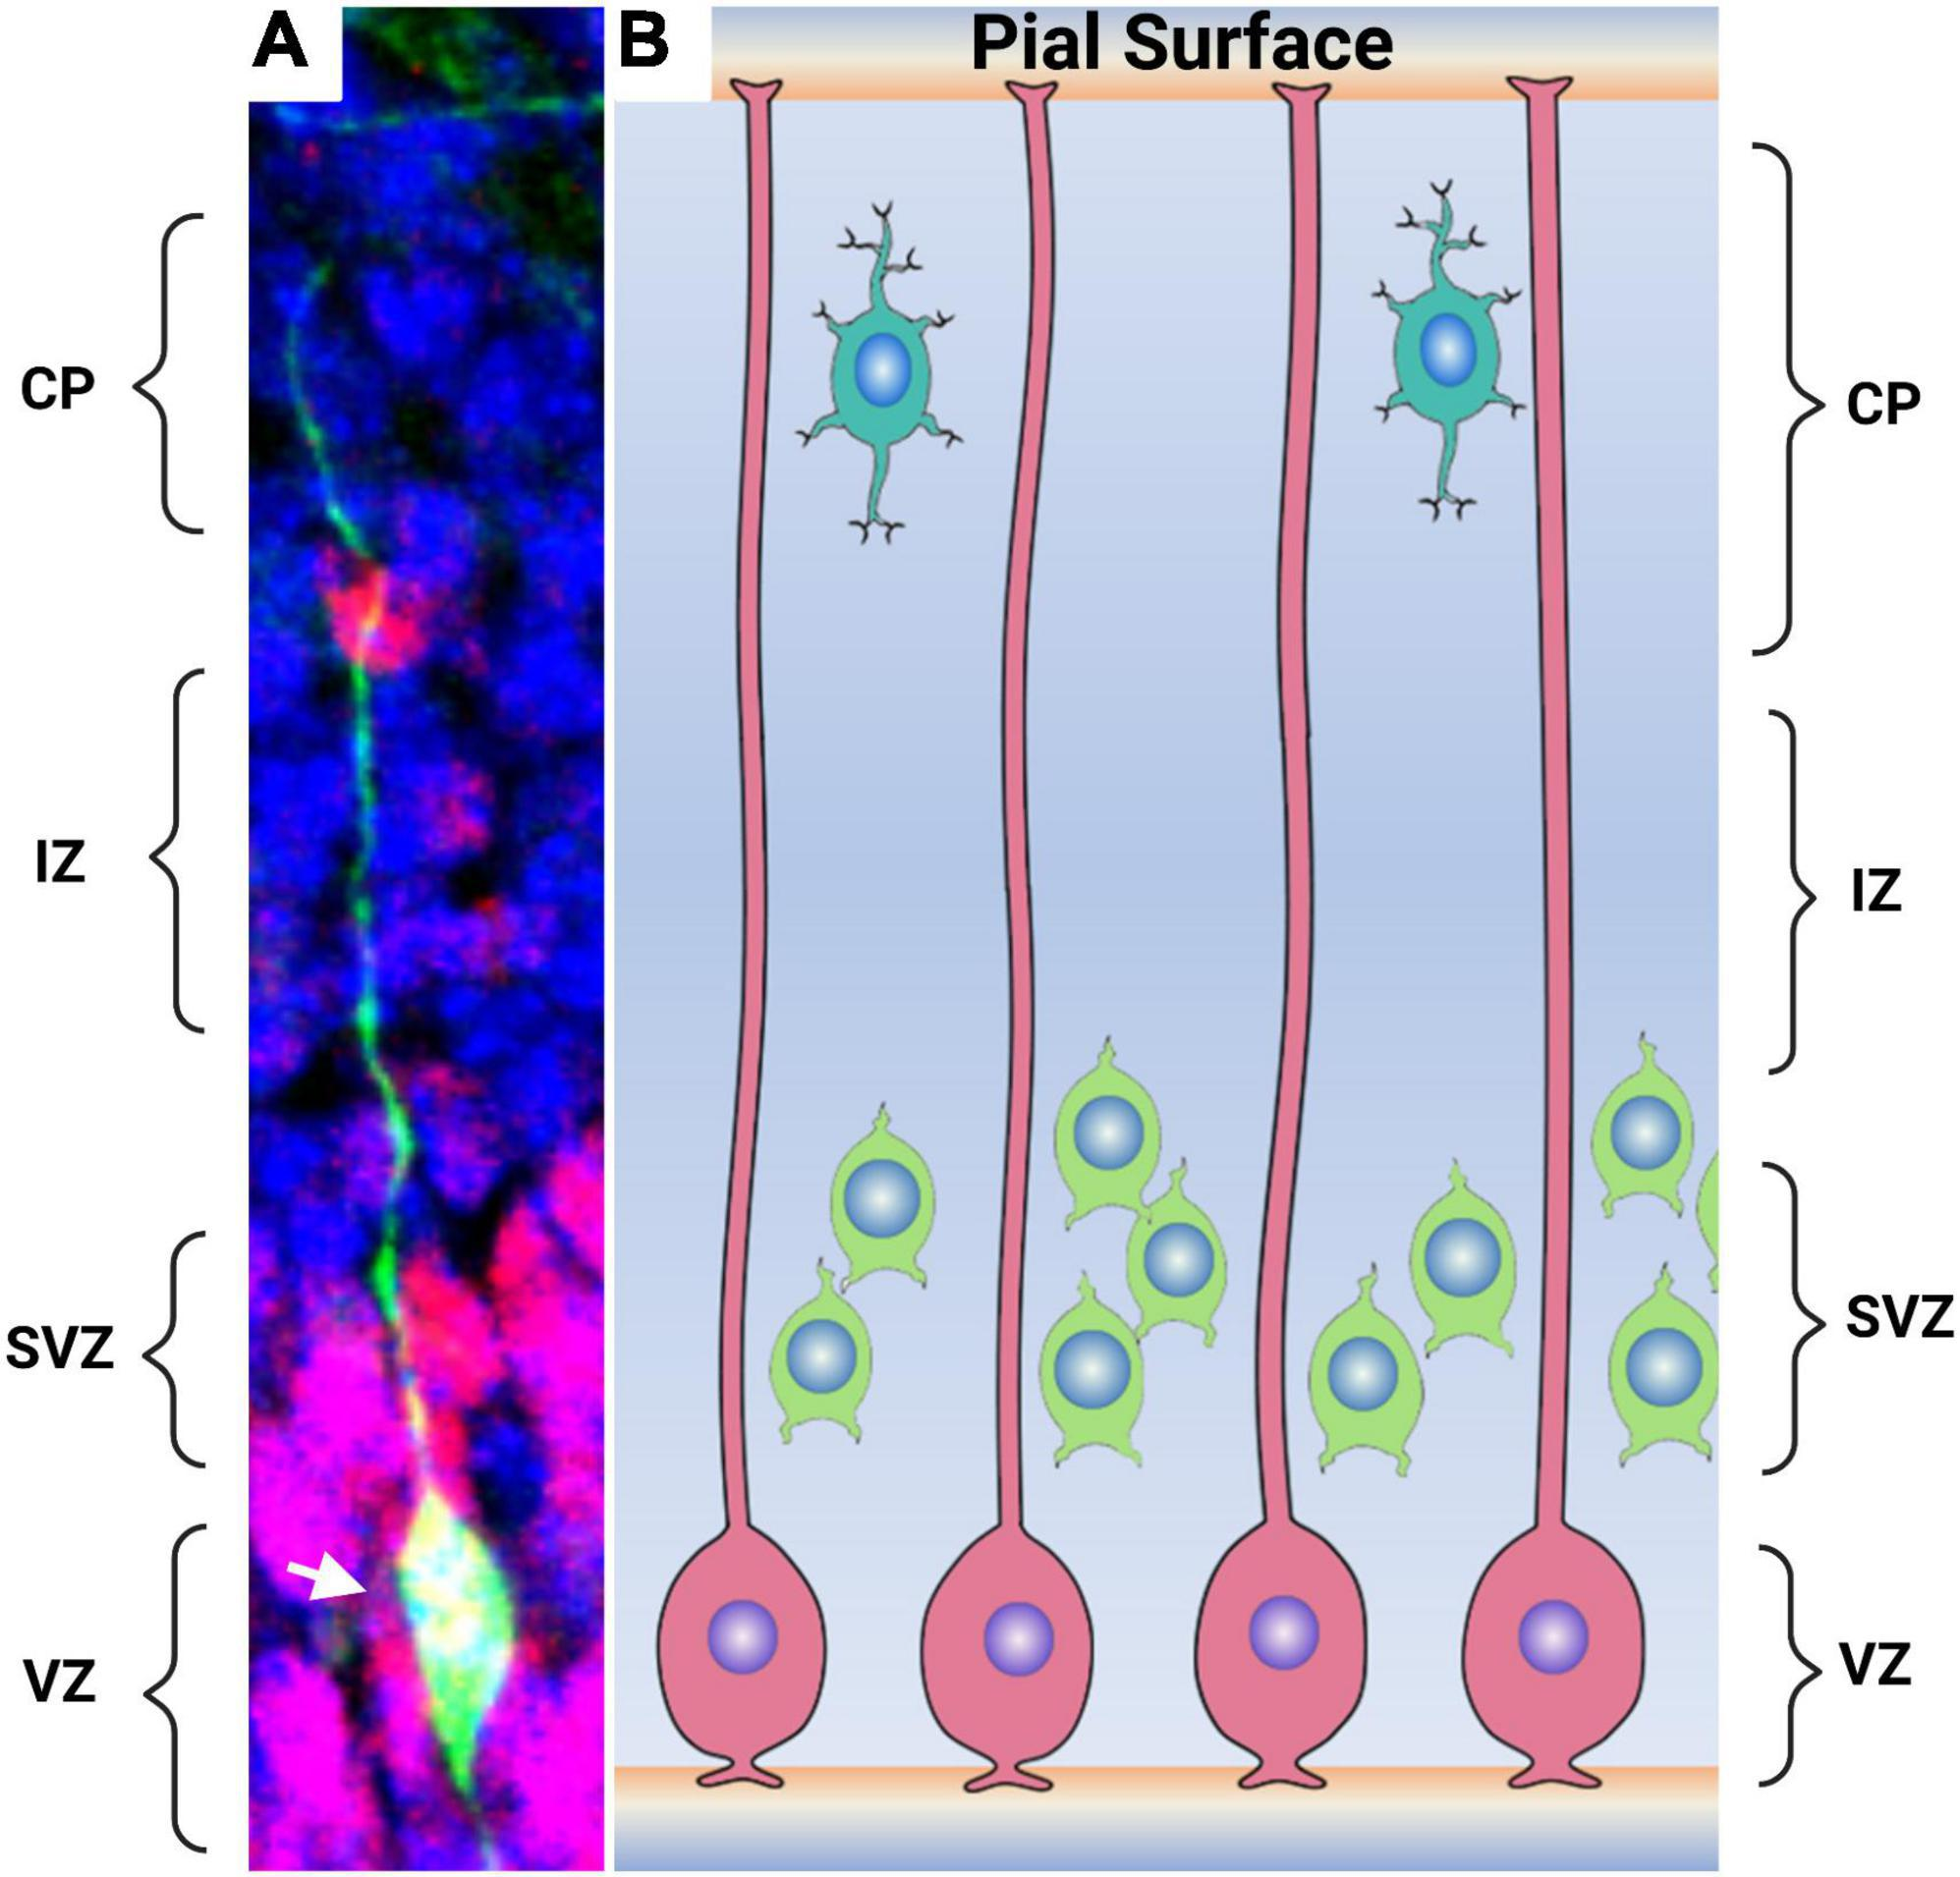
\includegraphics{images/neuro-radialglia.jpg}
\end{itemize}

\hypertarget{cuxe9lulas-de-schwann-e-oligodendruxf3citos}{%
\subsubsection*{Células de Schwann e oligodendrócitos}\label{cuxe9lulas-de-schwann-e-oligodendruxf3citos}}
\addcontentsline{toc}{subsubsection}{Células de Schwann e oligodendrócitos}

Esses tipos celulares são responsáveis por garantir uma condução mais eficiente e célere de impulsos elétricos através dos axônios neuronais por meio da \textbf{mielinização de fibras nervosas}, processo que possibilita a condução saltatória dos potenciais de ação por meio dos nós de Ranvier, pequenos intervalos de membrana desnuda interpostos entre as bainhas de mielina, áreas de revestimento lipídico eletrodinamicamente isolante. Essas células costumam apresentar poucas ramificações (conforme já se pode antever pela própria etimologia grega da palavra ``oligodendrócito''), as quais são primordiais para a fisiologia da mielinização na medida em que se enrolam repetidamente sobre os axolemas neuronais. Nesse âmbito, é necessário destacar que, ao passo que os \textbf{oligodendrócitos} são exclusivos do Sistema Nervoso Central e são capazes de mielinizarem vários axônios ao mesmo tempo, as \textbf{células de Schwann} podem ser observadas exclusivamente no Sistema Nervoso Periférico e podem mielinizar, cada uma, apenas um curto segmento de um dado axônio.

\begin{itemize}
\tightlist
\item
  fotomicrografias e esquemas mostrando as diferenças entre as células de Schwann e os oligodendrócitos
\end{itemize}

Como resultado desses enrolamentos, essas células gliais formam alguns marcos estruturais idetificáveis por meio da microscopia eletrônica de transmissão e muito úteis para o estudo ultraestrutural das doenças desmielinizantes. Estes correspondem ao \textbf{mesaxônio externo}, uma esprial de \textbf{linhas intraperiódicas} (delimitadas pelo espaço extracelular compreendido entre duas voltas sucessivas do prolongamento mielinizador), uma espiral de \textbf{linhas densas principais} (formadas por uma pequena quantidade de citoplasma dos prolongamentos das células mielinizadoras interposta entre dois folhetos internos da estrutura trilaminar de suas membranas plasmáticas, as quais se encontram quase fundidas) e um \textbf{mesaxônio interno}.

\begin{itemize}
\tightlist
\item
  eletromicrografia mostrando a ultraestrutura da bainha de mielina
\end{itemize}

Cabe ressaltar que o processo de mielinização é absurdamente complexo do ponto de vista da Biologia Celular. Resumidamente, seria possível afirmar que, para que a mielina resultante seja viável, são necessárias junções de conexão e de oclusão homotípicas e heterotípicas, proteínas transmembranares responsáveis por compactarem as diversas camadas da espiral formada pelo enrolamento do axônio nos prolongamentos das células mielinizantes (com especial destaque para a proteína zero de mielina e a proteína proteolipídica) e volumes residuais de citoplasma interrompendo a continuidade das linhas densas principais em alguns pontos, correspondendo às \textbf{incisuras de Schmidt-Lantermann}.

\begin{itemize}
\tightlist
\item
  boxe mostrando as incisuras de Schmidt-Lantermann e explicando hipóteses acerca de suas possíveis funções
\end{itemize}

Sob a óptica da Neuropatologia, tem-se que as principais doenças que afetam o processo de mielinização decorrem ou de autoimunidades contra proteínas nele envolvidas (como no caso da esclerose múltipla e da Síndrome de Guillain-Barré) ou de mutações nos genes que as codificam. Para se exemplificar esse último cenário, poderíamos pensar na doença de Charcot-Marie-Tooth ligada ao cromossomo X, onde há um defeito molecular na conexina 32 presente nas junções de comunicação homotípicas presentes nas céulas de Schwann, e na doença de Charcot-Marie-Tooth dos tipos 1B e 2, situação na qual anomalias na proteína zero de mielina levam a prejuízos na compactação das bainhas lipídicas formadas pelos prolongamentos mielinizantes.

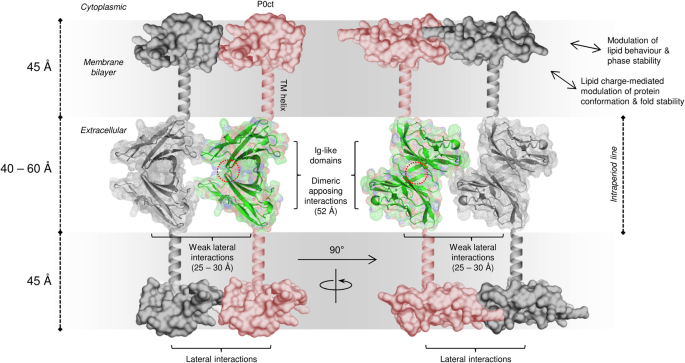
\includegraphics{images/neuro-p0myelin.png}
- imagens de estrutura proteica terciária computacional mostrando as proteínas zero de mielina ancorando-se entre dois folhetos de membrana plasmática adjacentes

\hypertarget{caso-cluxednico-raiva}{%
\section{Caso Clínico: Raiva}\label{caso-cluxednico-raiva}}

\hypertarget{cuxe9rebro}{%
\chapter{Cérebro}\label{cuxe9rebro}}

Anatomicamente, o cérebro pode ser considerado, sem sombra de dúvidas, a estrutura mais importante do Sistema Nervoso Central, podendo ser dividido em 47 áreas de Brodmann relacionadas aos mais diversos aspectos da experiência humana, tais como o processamento auditivo central, a empatia, a sensibilidade térmica e dolorosa, a linguagem, a cognição lógico-matemática, a personalidade e a memória. Além disso, temos também inúmeras estruturas subcorticais e diencefálicas vinculadas a mecanismos de analgesia, ao aprendizado motor e ao controle de funções vegetativas.

\begin{itemize}
\tightlist
\item
  mapa das áreas de Brodmann junto com legenda explicando as funções das principais delas
\end{itemize}

De uma perspectiva neuroembriológica, tem-se que o cérebro se desenvolve a partir da extremidade cefálica do tubo neural, formada a partir do fechamento do neuróporo rostral durante a quarta semana de desenvolvimento. Esse evento permite a formação de três vesículas encefálicas primárias, as quais correspondem, de rostral a caudalmente, ao \textbf{prosencéfalo}, ao mesencéfalo e ao rombencéfalo. Na quinta semana de desenvolvimento, o prosencéfalo se divide em duas vesículas encefálicas secundárias, correspondentes ao \textbf{telencéfalo}, o qual originará os hemisférios cerebrais, e ao \textbf{diencéfalo}. Deste são oriundas estruturas do:

\begin{itemize}
\tightlist
\item
  \textbf{tálamo}, o grande \emph{relé} sensitivo do Sistema Nervoso.
\item
  \textbf{metatálamo}, onde estão abrigados os corpos geniculados essenciais para as vias visual e auditiva.
\item
  \textbf{epitálamo}, onde se situa a glândula pineal.
\item
  \textbf{hipotálamo}, principal central de controle vegetativo do organismo.
\item
  \textbf{subtálamo}, fundamental para a frenagem de movimentos através da ativação da via indireta dos núcleos da base.
\end{itemize}

Nesse âmbito, é interessante mencionar que a \textbf{protuberância óptica} se desenvolve a partir do diencéfalo na sexta semana de desenvolvimento embrionário, o que justifica a sintopia mantida entre certas estruturas diencefálicas e os nervos ópticos, o quiasma óptico e os tratos ópticos.

No processo de histogênese do prosencéfalo, distinguem-se duas populações celulares primordiais: os \textbf{neuroblastos} e os \textbf{glioblastos}. Enquanto estes darão origem às populações celulares progenitoras dos gliócitos integrantes da macróglia (ou seja, os astroblastos e os oligodendroblastos), aqueles se diferenciarão sequencialmente em neuroblastos bipolares, neurblastos unipolares e neurônios. Vale salientar queé possível que aconteçam interconexões entre os processos de neurogênese e gliogênese, dentre as quais a \textbf{transformação gliogênica} se configura como mecanismo mais comum de conversão de neuroblastos em glioblastos. Finalmente, é preciso ressaltar que, no prosencéfalo, ocorre a migração dos neurônios originados na zona intermediária do tubo neural para a placa cortical, explicando a organização tecidual dos hemisféricos cerebrais num córtex composto por substância cinzenta, onde podem ser visualizados corpos celulares de neurônios, e num centro sensorial composto predominantemente por prolongamentos axônicos de tais neurônios corticais.

\begin{itemize}
\tightlist
\item
  esquema mostrando as diferentes zonas hitogenéticas do tubo neural.
\end{itemize}

No que tange à citoarquitetura dos circuitos neuronais complexos encontrados no córtex cerebral, vale mencionar que esta apresenta variações significativas conforme o grau de desenvolvimento filogenético da espécie estudada e a região cortical analisada. No entanto, é válido afirmar que, para todas as espécies, observa-se uma \textbf{organização laminar} das camadas de células do córtex cerebral, de modo que, usualmente, o córtex se encontra dividido em 6 camadas distintas. Quanto à classificação filogenética dessas regiões cerebrais, vislumbra-se uma subdivisão das áreas corticais em:

\begin{itemize}
\item
  \textbf{arquicórtex}, típico da formação hipocampal.
\item
  \textbf{paleocórtex}, característico do rinencéfalo e de áreas olfativas.
\item
  \textbf{neocórtex}, presente ao longo de 95\% de toda a extensão cortical, correspondendo ao território compreendido pelo isocórtex.
\item
  mapa filogenético do cérebro de diferentes espécies de mamíferos e animais em geral.
\end{itemize}

Por outro lado, sob uma perspectiva citoarquitetural, o córtex cerebral pode ser classificado como:

\begin{itemize}
\item
  \textbf{isocórtex}, quando estão presentes todas as camadas corticais, que são, de exterior para interior: a camada plexiforme ou molecular, a camada granular externa, a camada das células piramidais, a camada granular interna, a camada ganglionar e a camada das células multiformes.
\item
  \textbf{alocórtex}, no qual ao menos uma das seus camadas supramencionadas se faz ausente.
\item
  corte histológico impregnado por prata mostrando a organização das camadas do isocórtex.
\end{itemize}

O isocórtex ainda pode ser segmentado em três categorias, o que reflete o alto grau de especialização de diferentes áreas corticais para a efetuação dos mais variados tipos de tarefas e funções. Essas subcategorias são definidas com base no predomínio diferencial de uma camada cortical específica sobre as outras e compreendem as seguintes classificações:

\begin{itemize}
\tightlist
\item
  \textbf{isocórtex homotípico}, encontrado em áreas de associação e caracterizado por possuir estratos de espessuras similares entre si.
\item
  \textbf{isocórtex heterotípico agranular}, observado em áreas motoras primárias e secundárias e organizado de tal maneira que se nota um claro predomínio das camadas compostas por células piramidais sobre os demais estratos corticais.
\item
  \textbf{isocórtex heterotípico granular}, verificado em áreas sensitivas, nas quais existe uma dominância das camadas granulares sobre as outras.
\end{itemize}

Todavia, é preciso ressalvar que a boa visualização dessas camadas corticais e, por conseguinte, a classificação das áreas observadas de acordo com suas características citoarquiteturais e filogenéticas, só podem ser atingidas mediante o emprego de técnicas refinadas de imunofluorescência, as quais possibilitam a marcação dos tipos celulares típicos de cada estrato cortical de acordo com as proteínas expressas especificamente por cada um deles. Nesse contexto, é possível mencionar as seguintes populações celulares para cada lâmina do córtex cerebral:

\begin{itemize}
\item
  \textbf{Camada molecular}: nesse estrato cortical, há o predomínio de \textbf{prolongamentos axonais e dendríticos} de neurônios subjacentes, não sendo possível encontrar uma grande quantidade de células. Entretanto, ocasionalmente se pode deparar com gliócitos e \textbf{células horizontais de Cajal} (também denominadas células de Cajal-Retzius), neurônios glutamatérgicos e \(GABA\)érgicos fundamentais na mediação do processo de corticogênese via secreção de reelina, uma proteína sinalizadora morfogenética.
\item
  boxe com um esquema de sinalização celular mostrando a função da reelina e a importância dela para a embriologia.
\item
  \textbf{Camada granular externa}: essa camada se encontra composta por densas aglomerações de \textbf{células piramidais} e \textbf{células granulares}. Enquanto estas correspondem a neurônios multipolares do tipo II de Golgi e também são conhecidas como \textbf{células estreladas}, aquelas correspondem a neurônios multipolares do tipo I de Golgi e são os principais tipos de neurônios disparados na ativação do trato corticoespinal e na cognição.
\item
  \textbf{Camada das células piramidais (ou piramidal externa)}: nessa lâmina do córtex cerebral, nota-se um significativo predomínio de \textbf{células piramidais} com pericários de tamanho médio. Vale salientar que, como uma regra geral para essa população celular, observa-se que seus corpos celulares aumentam progressivamente de tamanho conforme mais profundamente se vai adentrando no córtex cerebral. Além dessas células, também se pode encontrar ocasionalmente \textbf{células de Martinotti}, pequenas células poligonais de prolongamentos dendríticos curtos relacionadas à inibição das atividades das células piramidais adjacentes, podendo, dessa maneira, desempenharem funções relevantes no controle motor.
\item
  \textbf{Camada granular interna}: esse estrato do córtex cerebral é constituído primariamente por \textbf{células estreladas} e é tido como a primeira camada cortical a receber aferências talâmicas, sendo, portanto, responsável por retransmiti-las às demais regiões do córtex. Em cortes do giro estriado (área 17 de Brodmann, também conhecida como área visual primária), é possível observar de modo nítido neurônios constituintes da via visual estabelecendo conexões com as células granulares da camada granular interna por meio das \textbf{fibras geniculocalcarinas}, as quais formam a Estria de Gennari, faixa esbranquiçada facilmente reconhecível à examinação macroscópica.
\item
  imagem de macroscopia mostrando a Estria de Gennari.
\item
  \textbf{Camada granular (ou piramidal interna)}: nessa região do plano estratimérico do córtex cerebral, pode-se visualizar grandes quantidades de \textbf{células piramidais} com somas de dimensões amplas e quantias consideráveis de células estreladas e de Martinotti. No giro pré-central, correspondente à área motora primária, essa camada abriga as \textbf{células de Betz}, os maiores neurônios de todo o Sistema Nervoso e as principais ativadoras de motoneurônios \u03B1 inferiores, estabelecendo sinapses excitatórias glutamatérgicas com estes e projetando-se por meio dos tratos corticoespinais lateral e anterior.
\item
  \textbf{Camada das células multiformes}: apresenta uma gama variada de populações celulares, abrigando células piramidais pequenas, células de Martinotti, células estreladas e \textbf{células fusiformes}. Estas apresentam morfologia alongada, porém, diferentemente das células horizontais de Cajal, dispõem-se perpendicularmente à superfície do córtex cerebral. As células fusiformes encontram-se funcionalmente relacionadas ao envio de impulsos neuronais para outras áreas corticais e para o tálamo.
\end{itemize}

Assim como outras estruturas do neuroeixo, o cérebro se encontra revestido por uma série de folhetos de tecido conjuntivo responsáveis por, dentre outras funções, fornecer proteção mecânica ao tecido nervoso, permitir a nutrição de seus componentes e promover a drenagem sanguínea do encéfalo por meio dos seios venosos. Tais membranas conjuntivas correspondem às meninges e, do ponto de vista estratimérico, elas correspondem, da mais externa para a mais interna, à \textbf{dura-máter}, à \textbf{aracnoide-máter} e à \textbf{pia-máter}.

A dura-máter se encontra aderida ao periósteo dos ossos da calota craniana no encéfalo e forma pregas responsáveis por compartimentalizarem a parte cefálica do paquímero dorsal do corpo, tais como a \textbf{foice do cérebro}, o \textbf{tentório do cerebelo} e a \textbf{foice do cerebelo}. Além disso, essa meninge é composta por um folheto externo e um folheto interno, os quais podem se separar em determinadas regiões para formarem importantes \textbf{seios venosos}, como os seios sigmoides, os seios transversos, o seio sagital superior e o seio sagital inferior, fundamentais para a drenagem venosa do parênquima encefálico.

Internamente à dura-máter, pode-se encontrar a aracnoide-máter, a qual é dividida numa parte mais externa que fica aderida à dura-máter e contribui para a formação de uma camada meníngea protetora espessa (a \textbf{paquimeninge}) e numa parte trabecular que se aprofunda em direção ao \textbf{espaço subaracnoideo}, principal reservatório de líquor cefalorraquidiano no Sistema Nervoso Central. De uma perspectiva histológica, pode-se dizer que a aracnoide-máter é composta fundamentalmente de tecido conjuntivo denso e \textbf{células meningoteliais} revestindo o espaço subaracnoideo.

\begin{itemize}
\tightlist
\item
  boxe explicando as funções das membranas serosas e do mesotélio e falando das células meningoteliais como possível quarto mesotélio do corpo.
\end{itemize}

Ainda mais internamente à aracnoide-máter, pode-se visualizar a pia-máter, o folheto meníngeo \textbf{mais delicado e vascularizado}, que se encontra intimamente aderida ao tecido nervoso e revestida por células meningoteliais de origem embrionária mesenquimatosa. Pelo espaço subaracnoideo transitam artérias dedicadas à irrigação de estruturas cerebrais e esses vasos adentram o parênquima encefálico por meio de canais revestidos por pia-máter e preenchidos por um delgado espaço fisicamente contíguo ao espaço subaracnoideo, denominado espaço perivascular ou \textbf{espaço de Virchow-Robbin}.

\begin{itemize}
\tightlist
\item
  diagrama (imagem de livro de Histologia ou Anatomia) mostrando a estrutura do espaço de Virchow-Robbin
\end{itemize}

\hypertarget{caso-cluxednico-meningoencefalite-criptocuxf3cica}{%
\section{Caso Clínico: Meningoencefalite criptocócica}\label{caso-cluxednico-meningoencefalite-criptocuxf3cica}}

\hypertarget{cerebelo}{%
\chapter{Cerebelo}\label{cerebelo}}

De uma perspectiva neuroanatômica, o cerebelo (cuja etimologia latina significa \emph{pequeno cérebro}) corresponde a um órgão do compartimento infratentorial especializado em mecanismos de \textbf{coordenação motora}, \textbf{aprendizado motor} e \textbf{correção dos movimentos corporais}, conectando-se com estruturas tais como o tálamo, o complexo olivar inferior bulbar, o córtex motor, o aparellho vestibular e a medula espinal. Morfologicamente, o cerebelo se situa posteriormente ao quarto ventrículo e se conecta com o tronco encefálico por meio de três pares de pedúnculos cerebelares (superior, médio e inferior), por onde trafegam vias e tratos neuronais responsáveis pelas mais variadas funções desse componente do Sistema Nervoso, que vão desde o planejamento motor junto às áreas 5 e 7 de Brodmann até papéis límicos relacionados à linguagem e à emoção.

Assim como o cérebro, o cerebelo tabmém apresenta uma camada cortical compreendida por substância cinzenta e uma camada medular composta primordialmente por substância branca, as quais correspondem, respectivamente, ao \textbf{córtex cerebelar} e ao \textbf{corpo medular do cerebelo} (denominado também \emph{árvore da vida} por apresentar uma geometria similar àquela observada nos galhos de uma árvore frondosa). Podem ser encontradas esturturas compostas por substância cinzenta mergulhadas no corpo medular, coletivamente referidas como \textbf{núcleos profundos do cerebelo}. Estes abrangem os núcleos \textbf{denteado}, \textbf{interpósito} (formado pela união dos núcleos \textbf{globoso} e \textbf{emboliforme}) e \textbf{fastigial}. Do ponto de vista da divisão longitudinal do cerebelo, cada núcleo se encontra relacionado a funções e vias específicas da motricidade, o que é de grande relevância clínica para a avaliação de quadros de lesões cerebelares no exame físico.

\begin{itemize}
\tightlist
\item
  boxe mostrando técnicas de avaliação das vias cerebelares no exame físico neurológico
\end{itemize}

Nesse âmbito, convém salientar que a \textbf{zona verminiana}, composta por uma estrutura altamente segmentada situada ao longo do plano sagital mediano e detentora de um formato parecido com o de uma minhoca (o que justifica seu nome). Essa região se relaciona primariamente com o \textbf{núcleo do fastígio}, estabelecendo conexões com o sistema vestibular por meio da via fastígio-vestibular, essencial para o ajuste de movimentos mediante alterações nas velocidades lineares e angulares do corpo.

Por outro lado, a \textbf{zona paraverminiana}, compreendida por boa parte dos hemisérios cerebelares, relaciona-se ao \textbf{núcleo denteado} e medeia processos vinculados à intercomunicação cérebro-cerebelo para o planejamento motor por intermédio da via eferente dento-tálamo-cortical e da via aferente córtico-ponto-cerebelar.

É necessário apontar que, assim como se pôde perceber para a classificação das regiões do córtex cerebral, o cerebelo também possui uma divisão filogenética, a qual guarda fortes correlações com os aspectos fisiológicos de cada uma de suas regiões. Destarte, é possível subdividir essa estrutura nervosa em:

\begin{itemize}
\tightlist
\item
  \textbf{arquicerebelo}: funcionalmente correlacionado com o vestibulocerebelo e constituído anatomicamente pelo lobo flóculo-nodular.
\item
  \textbf{paleocerebelo}: fisiologicamente relacionado ao espinocerebelo.
\item
  \textbf{neocerebelo}: vinculado ao cerebrocerebelo do ponto de vista funcional.
\end{itemize}

No que diz respeito à anatomia microscópica desse órgão, pode-se afirmar que seu plano estratimérico básico se caracteriza pela presença de uma camada cortical externa de substância cinzenta e uma camada medular interna de substância branca, sendo que o córtex cerebelar pode ser subdividido em três estratos, os quais correspondem, de mais exterior para mais interior, a uma \textbf{camada molecular}, uma camada de \textbf{células de Purkinje} e uma camada de \textbf{células granulosas}.

De modo análogo ao que é observado para a camada molecular do córtex cerebral, a camada molecular cerebelar é relativamente pobre em corpos celulares, porém \textbf{rica em prolongamentos neuronais}. Estes incluem os prolongamentos dendríticos extremamente ramificados das células de Purkinje e os prolongamentos axônicos das células granulosas, os quais se encontram sinapticamente acoplados. Dessa forma, a ativação das células granulares por meio de \textbf{fibras musgosas} provenientes de estruturas extracerebelares promove, consequentemente, a ativação das células de Purkinje. Essa circuitaria neuronal altamente regulada constitui um dos principais aspectos da citoarquitetura cerebelar que possibilitam o aprendizado motor por meio de ativações e silenciamentos sucessivos dos neurônios situados nos núcleos profundos do cerebelo, responsáveis por dispararem as vias eferentes previamente descritas. Dentre as raras populações celulares que possuem seus pericários situados na camada molecular do córtex cerebelar, pode-se elencar as \textbf{células estreladas} e as \textbf{células em cesta}. Estas últimas podem ser classificadas como neurônios multipolares do tipo II de Golgi, configurando-se como células inibitórias \(GABA\)érgicas que promovem a coordenaçãomotora ao inibirem as células de Purkinje e, consequentemente, suprimirem a inibição destas sobre os núcleos cerebelares profundos.

Já a camada de \textbf{células de Purkinje} é composta primariamente por neurônios multipolares do tipo I de Golgi com grandes corpos celulares e uma profusa ramificação dendrítica direcionada para a camada molecular. Essas células são umas das maiores de todo o organismo humano e exercem ação inibitória sobre os neurônios dos núcleos profundos do cerebelo por meio da liberação de \(GABA\) na fenda sináptica compreendida entre essas células ativadoras das vias cerebelares eferentes e os terminais axonais das células de Purkinje. Dessa forma, ocorre um influxo de íons Cl\textsuperscript{-} para o meio intracelular dos neurônios de tais núcleos, hiperpolarizando-os. As células de Pukinje são ativadas principalmente por meio da ação das \textbf{fibras trepadeiras}, que se originam do \textbf{núcleo olivar inferior} e emitem prolongamentos axônicos que parecem se entrelaçar helicoidalmente ao redor das fibras nervosas representadas pelos axônios das células de Purkinje, de modo similar ao que é constatado para as plantas epífitas, que parecem se enrolar ao redor dos troncos das árvores com as quais estabelecem relações ecológicas desarmônicas.

Por fim, cabe salientar que a \textbf{camada granulosa} do córtex cerebelar é composta primordialmente por \textbf{células granulosas}, neurônios multipolares do tipo Golgi I que emitem extensos prolongamentos axônicos retilíneos e amielínicos para a camada molecular do córtex cerebelar, e \textbf{células de Golgi}, as quais correspondem a interneurônios inibitórios \(GABA\)érgicos ativados pelas fibras musgosas e responsáveis por suprimirem as atividades das células granulosas. Teoriza-se que o papel das células de Golgi no contexto das intrincada circuitaria neural cerebelar esteja voltado à \textbf{plasticidade neuronal} no córtex cerebelar e ao rearranjo espaço-temporal dos níveis de atividade das células granulosas e de suas conexões sinápticas.

\begin{itemize}
\item
  boxe de biologia celular explicando os mecanismos moleculares subjacentes à plasticidade neuronal.
\item
  boxe fisiológico explicando os papéis desempenhados pelas fibras musgosas e a neuroanatomia delas.
\end{itemize}

\hypertarget{plexo-coroide}{%
\chapter{Plexo Coroide}\label{plexo-coroide}}

Sob uma óptica histológica, pode-se asserir que a população celular mais representativa das regiões nas quais se faz presente o plexo coroide corresponde às \textbf{células ependimárias}, embriologicamente derivadas das células ventriculares que povoam a zona ventricular do tubo neural durante o processo de histogênese do tecido nervoso. Além de tais células, também é possível encontrar \textbf{tanicitos} em algumas regiões específicas do sistema ventricular encefálico, os quais correspondem a células derivadas da glia radial bipolar detentoras de uma morfologia intermediária entre os astrócitos e as células ependimárias. Dessa forma, é válido frisar que as células ependimárias e os tanicitos constituem os principais componentes neuroepiteliais do epêndima, imprescindível para a produção e a movimentação do líquido cefalorraquidiano.

\begin{itemize}
\item
  boxe de Biologia Celular mostrando imagens de imunofluorescência das células ependimárias e dos tanicitos e explicando as diferenças de morfologia, com enfoque para a morfologia estranha dos tanicitos.
\item
  boxe anatômico mostrando os componentes do sistema ventricular do Sistema Nervoso, ou seja, desde as cisternas até os ventrículos em si e os aquedutos que os conectam.
\item
  esquema de histogênese do tecido nervoso explicado por zonas do tubo neural (pode ser aquela do Kierszenbaum)
\end{itemize}

Como já se pode inferir a partir das populações celulares gliocíticas descritas acima, o plexo coroide (ou corioide) corresponde a uma associação de \textbf{estruturas circumventriculares} e um \textbf{epêndima} de características epitelioides que abriga células especializadas na produção do líquor a partir do plasma sanguíneo. Nesse sentido, é pertinente lembrar que os chamados \emph{órgãos circumventriculares} são regiões do Sistema Nervoso Central nas quais se observam descontinuidades da barreira hematoencefálica e, dessa forma, representam áreas de fluxo de substâncias facilitado entre o meio intravascular e o tecido nervoso. Do ponto de vista ultraestrutural, o plexo coroide constitui-se essencialmente pela interface entre uma rede de capilares fenestrados com diafragma situada no interior de uma massa de tecido conjuntivo frouxo e o epêndima sobrejacente.

\begin{itemize}
\tightlist
\item
  mostrar fotomicrografia lâmina de plexo coroide indicando os componentes histológicos de suas estruturas.
\end{itemize}

Assim, pode-se dizer que o plexo coroide está presente nas paredes do terceiro e do quarto ventrículos, onde uma película fina de \textbf{pia-máter} altamente vascularizada denominada \textbf{tela coroide} oferece o aporte sanguíneo necessário para a produção de líquor e, nas fissuras coroides dos ventrículos laterais, situadas nas seções mediais desses componentes do sistema ventricular encefálico, entre o fórnice e o tálamo. Nessas regiões verifica-se, além da intensa produção de líquor, um incisivo e perene \textbf{monitoramento imunológico} por parte de macrófagos, linfócitos e células dendríticas encontradas no tecido conjuntivo frouxo que sustenta o plexo coroide.

\begin{itemize}
\tightlist
\item
  boxe fisiológico versando sobre a importância das células do Sistema Imunológico inclusas no plexo coroide.
\end{itemize}

Ultraestruturalmente, as células ependimárias apresentam grandes quantidades de \textbf{mitocôndrias} e múltiplas \textbf{invaginações basais} de seus domínios de membrana basolaterais, fatores que as caracterizam como células detentoras de intensa atividade metabólica e elevadas taxas de transporte ativo ocorrendo por bombas proteicas incrustadas na membrana plasmática. Ademais, a presneça de \textbf{microvilosidades} e eventuais \textbf{cílios} em seus domínios de membrana apicais é significativa do ponto de vista histofisiológico, haja vista que as células em questão também efetuam a absorção e a circulação do líquor. Finalmente, é interessante apontar a existência de uma resistente \textbf{barreira hematoliquórica} constituída por junções de oclusão e interdigitações estabelecidas entre células ependimárias adjacentes. Tais especializações laterias de membrana são, pois, fundamentais para se evitar a passagem direta de moléculas do sangue para o líquido cefalorraquidiano.

\begin{itemize}
\tightlist
\item
  boxe ultraestrutural mostrando eletromicrografia de transmissão do epênima, evidenciando os capilares fenestrados com diafragma que circulam pelo estroma e a Biologia Estrutural das barreiras hematoencefálica (fazer comparativo com outro corte, porque ela não vai estar presente aqui) e hematoliquórica.
\end{itemize}

\hypertarget{medula-espinal}{%
\chapter{Medula Espinal}\label{medula-espinal}}

De uma perspectiva neuroanatômica, a medula espinal se constitui como um grande \textbf{\emph{conduit} neuronal} central responsável por integrar o encéfalo com os compontnes do Sistema Nervoso Periférico. Isso possibilita, por exemplo, que o núcleo rubro medeie o controle ultrapreciso da musculatura intrínseca da mão por meio do trato rubroespinal, e que o sistema límbico receba e processe informações aferentes de dor crônica captadas por fibras nociceptivas amielínicas do tipo C na periferia do corpo e transmitidas ao prosencéfalo pro meio da \textbf{via paleoespinotalâmica}.

\begin{itemize}
\tightlist
\item
  boxe clínico sobre a relevância da via paleoespinotalâmica na patogenia da depressão.
\end{itemize}

Convém, entretanto, frisar que as características fisiológicas da medula espinal vão muito além do que aquelas que se poderia esperar de um simples cilindro constituído puramente por prolongamentos axônicos responsáveis por carregarem \emph{inputs} oriundos dos tecidos periféricos e \emph{outputs} para estes dirigidos. Desse modo, verifica-se que a medula espinal também está envolvida no controle das funções vegetativas do organismo por meio dos \textbf{núcleos intermédio-laterais} toracolombares e dos \textbf{núcleos intermédio-mediais} sacrais, em mecanismos de analgesia mediados pela \textbf{Substãncia Gelatinosa de Rolando} e até mesmo em arcos reflexos altamente intrincados, com a ativação e a inibição de grupamentos musculares inteiros. Nesse âmbito, é interessante ressaltar que o fenômeno da modulação negativa da dor por meio de estímulos táteis, explicado pela \textbf{Teoria da Comporta da Dor}, ocorre ao nível da medula espinal e hodiernamente é alvo de múltiplos estudos que visam à invenção de novos tratamentos farmacológicos da dor crônica.

\begin{itemize}
\tightlist
\item
  boxe farmacológico sobre o sistema opioide endógeno, a fisiologia da teoria da comporta da dor e atividades do cotidiano que liberam opioides endógenos.
\end{itemize}

Macroscopicamente, a medula espinal apresenta como limite superior a \textbf{decussação das pirâmides} e como limite inferior o \textbf{ligamento coccígeo}, originado a partir da parte dural do \textbf{filamento terminal}, emitido a partir do \textbf{cone medular}. A medula espinal apresenta uma organização metamérica, que, no entanto, é díspar daquela observada para a coluna vertebral, estojo ósseo que delimita a parte caudal do paquímero dorsal e abriga a estrutura nervosa em questão. Isso se dá em decorrência das taxas de crescimento diferenciais observadas para essas duas estruturas durante o processo de organogênese, de tal forma que é válido afirmar que um determinado segmento vertebral abriga estruturas nervosas referentes ao metâmero espinal dois níveis inferiores a ele. Assim, na seção do canal vertebral compreendida pela vértebra T\(V\), é possível encontrar o segmento medular T7.

\begin{itemize}
\item
  esquema mostrando as taxas de crescimento diferencial da medula e da coluna vertebral.
\item
  desenho mostrando a anatomia mmacroscópica da medula espinal.
\end{itemize}

Diferentemente do que se verifica para o encéfalo, a medula apresenta uma estratimeria na qual a \textbf{substância branca} composta majoritariamente por células da glia e prolongamentos axônicos ascendentes e descendentes se encontram na \textbf{periferia} do tubo e a \textbf{substância cinzenta}, compreendida por gliócitos e corpos celulares de neurônios, encontra-se numa posição \textbf{central}. Isso se dá naturalmente mediante o processo de histogênese do órgão em questão, o qual se desenvolve a partir do tubo neural, cujo lúmen se oblitera quase completamente nesse processo. É interessante apontar que a divisão clássica da substância cinzenta do \emph{H} medular num \textbf{corno ventral eferente motor} e um \textbf{corno dorsal aferente sensitivo} possui fundamentação embriológica. Ao passo que este é oriundo de uma estrutura denominada \textbf{placa alar}, a qual se forma por meio das células constituintes da parede dorsal do tubo neural e se diferencia em estruturas nervosas sensitivas por meio da ação do morfógeno \(Wnt\), aquele é originado a partir da \textbf{placa basal}, que se desenvolve a partir da parede ventral do tubo neural e se diferencia em neurônios motores inferiores através da indução morfogenética efetuada pela proteína \(SHH\) em suas células. Nesse sentido, pode-se lembrar que, diferentemente do que se observa na medula de um indivíduo que já completou seu desenvolvimento embrionário, a medula primitiva apresenta sulcos laterais responsáveis por demarcar o limite entre as placas alares e as placas basais, denominados \textbf{sulcos limitantes}.

\begin{itemize}
\item
  boxe embriológico sobre a ação morfogenética das proteínas \(SHH\) e \(Wnt\) e seus papéis na organogênese.
\item
  esquema ilustrando o processo de desenvolvimento supradescrito.
\end{itemize}

Outro aspecto anatômico no qual se pode notar claras diferenças entre as organizações macroscópicas e mesoscópicas do encéfalo e da medula espinal se dá na organização dos folhetos meníngeos, uma vez que, na medula, a dura-máter não se encontra aderida ao periósteo das vértebras, apresentando-se relativamente solta no interior do canal vertebral, formando o \textbf{saco dural}, uma estrutura fibrosa de \textbf{tecido conjuntivo denso} responsável por fornecer proteção mecânica à medula. Externamente ao saco dural, é possível observar a presença de tecido conjuntivo frouxo, tecido adiposo unnilocular e elementos neurovasculares preenchendo o \textbf{espaço epidural}. Vale salientar que, dentre as estruturas vasculares que podem ser encontradas nessa região, tem-se o \textbf{plexo venoso de Batson}, o qual promove a drenagem sanguínea da medula espinal e se conecta com veias das cavidades torácica e abdominopélvica. Tais conexões explicam o porquê de certos tipos de neoplasias, como o câncer de próstata, efetuarem metástases hematogênicas parao Sistema Nervoso Central.

\begin{itemize}
\tightlist
\item
  boxe anatômico e clínico destacando os diferentes espaços delimitados pelos folhetos meníngeos e a relevância deles na Anestesiologia.
\end{itemize}

Microscopicamente, é possível subdividir a substância cinzenta da medula espinal, que se dispõe num formato parecido com uma letra \emph{H} ou com uma borboleta (ganhando, por isso, a denominação de \emph{H} medular), em uma série de \textbf{lâminas} ou \textbf{núcleos} conhecidos como \textbf{lâminas de Rexed}. Cada uma dessas lâminas desempenha papéis específicos na modulação das atividades dos tratos espinais que trafegam pela substância branca e nas funções motoras e sensitivas desempenhadas pelo neuroeixo em sua interface de integração com o restante do organismo por meio do Sistema Nervoso Periférico. É interessante ressaltar que a proporção entre as áreas ocupadas pela substância cinzenta e pela substância branca aumenta craniocaudalmente, de forma que a medula espinal sacral possui um predomínio de substância cinzenta e a medula espinal cervical, de substância branca.

\begin{itemize}
\tightlist
\item
  Boxe embriológico e fisiológico sobre a biologia do desenvolvimento das lâminas de Rexed e as funções de cada uma delas.
\end{itemize}

\hypertarget{nervos}{%
\chapter{Nervos}\label{nervos}}

A partir de uma óptica neuroanatômico, é válido afirmar que os nervos são as principais estruturas que compõem o \textbf{Sistema Nervoso Periférico} e, por isso, funcionam como \emph{fios} que abrigam importantes circuitos neuronais responsáveis pela comunicação entre o Sistema Nervoso Central e as demais regiões do corpo. Isso possibilita que o Sistema Nervoso como um todo atue, ao lado do Sistema Endócrino, como uma rede de integração entre os múltiplos órgãos das várias regiões do corpo.

\begin{itemize}
\item
  boxe traçando um paralelo entre a estrutura de um computador e a morfofisiologia do sistema nervoso.
\item
  boxe sobre os chamados \emph{sistemas de integração} e a importância deles para a manutenção da homeostase, se possível falar de como sua fisiologia pode ser modelada pela Biologia de Sistemas do ponto de vista matemático.
\end{itemize}

Ao todo, possuímos \textbf{12 pares de nervos cranianos} e \textbf{31 pares de nervos espinais}. Enquanto estes se originam a partir da substância cinzenta do \emph{H} medular, aqueles se originam de núcleos imersos na substância branca do \textbf{tronco encefálico}, a exemplo do nervo vago (NC X), o qual se origina parcialmente do núcleo dorsal motor do nervo vago, e do nervo oculomotor (NC III), que possui seu componente autonômico oriundo do núcleo de Edinger-Westphal, ou de \textbf{projeções telencefálicas} e \textbf{diencefálicas}, como se observa para o nervo olfatório (NC I) e o nervo óptico (NC II), respectivamente.

\begin{itemize}
\tightlist
\item
  boxe clínico sobre a avaliação dos nervos cranianos no exame físico neurológico.
\end{itemize}

De forma geral, pode-se dizer que todo nervo possui um componente \textbf{aferente sensitivo} e um componente \textbf{eferente motor} e, do ponto de vista histológico, compõe-se por conjuntos de prolongamentos axônicos revestidos por membranas protetivas de tecido conjuntivo e fibras colágenas. Tais prolongamentos podem ou não estar mielinizados e isso dependerá da atividade das \textbf{células de Schwann}, os principais gliócitos do Sistema Nervoso Periférico. Essas células apresentam \textbf{núcleos sinuosos e alongados} que parecem acompanhar as trajetórias percorridas pelos prolongamentos nervosos.

\begin{itemize}
\tightlist
\item
  eletromicrografia das células de Schwann.
\end{itemize}

Os nervos usualmente podem ser encontrados em estreita associação com elementos vasculares tais como as veias de médio calibre e as artérias musculares constituintes dos \textbf{feixes vásculo-nervosos}, e se encontram compartimentalizados em \textbf{feixes} e \textbf{fascículos} nervosos por meio das membranas conjuntivas supramencionadas. Estas correspondem ao \textbf{epineuro}, ao \textbf{perineuro} e ao \textbf{endoneuro}.

Nesse âmbito, é possível mencionar que, enquanto o \textbf{epineuro} une vários fascículos nervosos em um só nervo e é composto primordialmente por \textbf{tecido conjuntivo denso}, o \textbf{perineuro} delimita os fascículos nervosos e corresponde a uma bainha conjuntiva constituída por uma série de fibroblastos modificados com formato achatado entremeados por fibras colágenas. Existe ainda o \textbf{endoneuro}, que corresponde a uma delicada película de \textbf{tecido conjuntivo frouxo} que reveste fibras nervosas individuais.

\begin{itemize}
\tightlist
\item
  esquema mostrando a estrutura dos folhetos de revestimento dos nervos ao lado de uma fotomicrografia legendada deles.
\end{itemize}

Entre os fascículos nervosos, pode-se observar, no interior das bainhas conjuntivas supradescritas, \textbf{vasos sanguíneos} responsáveis pela vascularização do tecido nervoso periférico. Vale salientar que os nervos configuram-se como estruturas de notável relevância clínica no exame físico neurológico, podendo ser lesados por uma miríade de afecções com as mais variadas etiologias, como a hanseníase, a neuropatia diabética e a esclerose múltipla.

\begin{itemize}
\tightlist
\item
  boxe microbiológico sobre a hanseníase e os mecanismos de virulência subjacentes aos danos causados em ramos nervosos sensitivos pelo \emph{Mycobacterium leprae}.
\end{itemize}

\hypertarget{guxe2nglios}{%
\chapter{Gânglios}\label{guxe2nglios}}

\hypertarget{guxe2nglios-sensitivos}{%
\section{Gânglios Sensitivos}\label{guxe2nglios-sensitivos}}

As fibras sensitivas constituintes dos nervos espinais apresentam seus somas situados em dilatações localizadas na \textbf{raiz dorsal} de seus nervos, em estruturas conhecidas como \textbf{gânglios sensitivos das raízes dorsais}. Esses neurônios pseudounipolares transmitem informações sensitivas ao Sistema Nervoso Central por meio das vias \textbf{coluna dorsal-lemnisco medial}, responsável pela condução de informações relacionadas ao tato epicrítico, à sensibilidade vibratória e à propriocepção consciente de todo o corpo com exceção da cabeça e do pescoço, e \textbf{anterolateral}, a qual conduz informações relacionadas ao tato protopático, à propriocepção inconsciente, à nocicepção e à termocepção.

\begin{itemize}
\item
  Boxe fisiológico e farmacológico sobre os anestésicos locais e a fisiologia das células nociceptivas.
\item
  Boxe histórico sobre a Lei de Hilton e a Lei da Energia Específica dos Nervos.
\end{itemize}

Como característica histológica peculiar dos gânglios sensitivos, é possível mencionar a presença de gliócitos especializados, denominados \textbf{células satélites}, ``contornando'' e sustentando os corpos celulares e os neuritos dos neurônios sensitivos. Ao emitirem um prolongamento centrípeto em direção à medula espinal e um prolongamento centrífugo em direção à periferia do organismo, os gânglios sensitivos proporcionam a integração somatossensorial entre diferentes regiões do corpo, o que é de especial importância para a defesa do organismo e para a mediação de \textbf{arcos reflexos}.

\begin{itemize}
\tightlist
\item
  boxe fisiológico sobre a Fisiologia dos arcos reflexos e as manobras de testagem de reflexos mais relevantes no exame físico neurológico.
\end{itemize}

\hypertarget{guxe2nglios-autonuxf4micos}{%
\section{Gânglios Autonômicos}\label{guxe2nglios-autonuxf4micos}}

Essas estruturas integram a \textbf{divisão visceral} do Sistema Nervoso e são fundamentais para o controle das funções vegetaticas, estabelecendo conexões com os gânglios pré-vertebrais simpáticos, os gânglios das cadeias paravertebrais e os núcleos intermédio-mediais da medula espinal. Nesse sentido, vale salientar que, nas lâminas observadas, verifica-se a presença dessas estruturas no \textbf{Sistema Nervoso Entérico}, onde formam o \textbf{plexo mioentérico} (ou de \textbf{Auerbach}), situado entre as camadas musculares circular interna e longitudinal externa do intestino e envolvido na regulação da motilidade destas, e o \textbf{plexo submucoso} (ou de \textbf{Meissner}), localizado na camada submucosa e essencial para o controle da motilidade do estrato muscular da mucosa e para o controle quimioceptivo e mecanoceptivo da peristalse.

\begin{itemize}
\tightlist
\item
  Boxe de biologia celular versando sobre a importância do SNE na patogenia de doenças psíquicas e sobre as principais funções dele.
\end{itemize}

Ainda se pode vislumbrar a presneça de pequenos gânglios autonômicos em meio ao tecido conjuntivo presente nas trabéculas da \textbf{glãndula submandibular}, onde medeia suas atividades secretórias conectando-se com fibras provenientes do nervo facial.

\hypertarget{aplicauxe7uxe3o-cluxednica}{%
\section{Aplicação Clínica}\label{aplicauxe7uxe3o-cluxednica}}

O vírus causador da \emph{Herpes zoster} tende a se alojar nos gânglios sensitivos das raízes dorsais dos nervos espinais quando se converte em seu estado latente após uma primoinfecção. Assim, mediante episódios de imunossupressão intensa, esse patógeno pode voltar à sua forma ativa e proporcionar o aparecimento de feridas máculo-papulares e vesiculares que se distribuem metamericamente na superfície do corpo, obedecendo os padrões de delimitação dos \textbf{dermátomos}. Cabe ressaltar que essas lesões podem ser desencadeadas por estresse emocional severo e podem ulcerar se deixadas sem tratamento, o que favorece a ocorrência de infecções secundárias.

\begin{itemize}
\tightlist
\item
  Boxe anatômico e embriológico sobre os dermátomos e os gradientes morfogenéticos que estão por trás de sua origem no desenvolvimento.
\end{itemize}

\hypertarget{mecanorreceptores}{%
\chapter{Mecanorreceptores}\label{mecanorreceptores}}

\hypertarget{corpuxfasculos-de-vater-paccini}{%
\section{Corpúsculos de Vater-Paccini}\label{corpuxfasculos-de-vater-paccini}}

Os corpúsculos de Vater-Paccini correspondem a estruturas nervosas encapsuladas por \textbf{lamelas concêntricas} de tecido conjuntivo e responsáveis pela detecção de informações relacionadas à \textbf{sensibilidade vibratória} e à \textbf{pressão} exercida em \textbf{camadas profundas} da derme reticular e na hipoderme, onde tais estruturas componentes do Sistema Somatossensorial são mais numerosas. Por possuírem um complexo revestimento de fibras colágenas entremeadas por fluido intersticial, esses receptores são sensíveis até mesmo às mais sutis variações da pressão aplicada sobre a superfície da pele, encontrando-se distribuídos em abundância por regiões do tegumento recobertas por pele espessa e sujeitas a atritos e forças friccionais intensas e constantes, a exemplo da palma da mão e da superfície plantar do pé.

Convém, todavia, salientar que essas terminações nervosas mecanorreceptoras não são exclusivas do Sistema Tegumentar, podendo também ser visualizadas em vísceras secretoras como o \textbf{pâncreas}, em \textbf{articulações} e no \textbf{periósteo} que reveste os componentes ósseos do esqueleto. Não se sabe ao certo os papéis fisiológicos efetuados pelos corpúsculos de Vater-Paccini nestes locais, especialmente no que concerne à população desses mecanorreceptores encontrada nas trabéculas conjuntivas do pâncreas. Entretanto, é teorizado que eles possam estar envolvidos no controle central da secreção realizada por essa importante glândula anfícrina retroperitoneal por meio da detecção de variações na pressão hidrostática no interior dos ductos secretores ao decorrer da ejeção do suco pancreático para a porção descendente do duodeno.

\begin{itemize}
\tightlist
\item
  boxe fisiológico sobre a a viscerocepão e o papel dos mecanorreceptores nisso tudo.
\end{itemize}

De um ponto de vista neurofisiológico, é possível afirmar que as informações captadas pelos corpúsculos de Paccini chegam ao \textbf{córtex somatossensorial primário}, correspondente ao \textbf{giro pós-central} (áreas 1, 2 e 3 de Brodmann), por meio da via \textbf{coluna dorsal-lemnisco medial}. Nesse âmbito, observa-se que o primeiro neurônio da via, cuja terminação nervosa periférica forma o corpúsculo de Paccini, possui seu pericário situado nos \textbf{gânglios sensitivos das raízes dorsais} dos nervos espinais e, ao adentrar na medula, envia um longo prolongamento axônico para o \textbf{tálamo} por meio do \textbf{funículo posterior} da substância branca medular. Particularmente, verifica-se que há um expressivo direcionamento das fibras nervosas para núcleos talâmicos responsáveis pela retransmissão das informações referentes à sensibilidade vibratória, à propriocepção consciente e ao tato epicrítico, merecendo destaque os núcleos \textbf{ventral póstero-lateral} e \textbf{ventral póstero-medial}.

\begin{itemize}
\tightlist
\item
  esquema mostrando a via da coluna dorsal-lemnisco medial
\end{itemize}

Ao chegar nesses centros talâmicos, o impulso nervoso é retransmitido para a \textbf{camada IV (granular interna)} do córtex somatossensorial primário, onde obedece um padrão de distribuição \textbf{somatotópico}

\begin{itemize}
\tightlist
\item
  boxe embriológico e anatômico falando sobre os mapas corticais para somatotopia e tonotopia e a origem desses mapas do ponto de vista da biologia do desenvolvimento.
\end{itemize}

\hypertarget{botuxf5es-gustativos}{%
\chapter{Botões Gustativos}\label{botuxf5es-gustativos}}

Histologicamente, essas \textbf{estruturas neuroepiteliais} formam pequenos aglomerados elipsoides de células incrustadas no epitélio pavimentoso estratificado não-queratinizado característico da mucosa de revestimento especializada da língua, podendo ser encontrados nas superfícies das papilas \textbf{fungiformes}, \textbf{foliáceas} e \textbf{circunvaladas} (a exceção são as papilas filiformes, que cumprem funções mais relacionadas à fricção do alimento com a superfície lingual do que à sensibilidade espacial gustatória). Nessas estruturas neuroepiteliais, é possível distinguir a existência de três populações celulares:

\begin{itemize}
\item
  As células \textbf{basais}, que funcionam como células-tronco e se encontram destinadas à reposição contínua das células gustativas.
\item
  Já as \textbf{células gustativas} são especializadas na detecção de sabores por meio do reconhecimento de moléculas solúveis dispersas na saliva e se degradam muito rapidamente quando comparadas a outras populações celulares, haja vista suas meias-vidas estimadas de 5 a 10 dias. Cabe ressaltar que essas células são providas de abundantes microvilos apicais que usualmente dispõem de grandes quantidades de receptores metebotrópicos dedicados à percepção dos sabores liberados pela comida e à transdução de sinais elétricos por estes proporcionados.
\item
  boxe de biologia molecular sobre proteínas da família TRPV e de seus papeis na detecção de sabores
\item
  Por fim, as \textbf{células sustentaculares} são responsáveis pela sustentação das populações celulares supramencionadas, atuando como um componente estromal dos botões gustativos.
\end{itemize}

Nesse âmbito, também é válido mencionar que as células gustativas receptoras se encontram divididas em \textbf{3 subtipos} principais, cada qual dedicado à percepção de diferentes modalidades gustativas. Assim, tem-se que, ao passo que as células gustativas do \textbf{tipo I} se encontram especializadas na captação de informações relativas ao sabor salgado, as células gustativas do \textbf{tipo II} estão voltadas à detecção do doce, do \emph{umami} (sabor característico de alimentos ricos em glutamato, tais como o peixe cru, os cogumelos e alguns tipos de queijo) e do amargo por meio de receptores metabotrópicos denominados \textbf{transducinas}. Finalmente, tem-se que as células gustatórias do \textbf{tipo III} possuem propriedades características de células excitáveis, sendo capazes de conduzir potenciais de ação e desempenharem respostas elétricas vinculadas aos sabores azedo e salgado por intermédio de despolarizações proporcionadas pela entrada de cátions (Na\textsuperscript{+} e Ca\textsuperscript{2+}) através de canais iônicos voltagem-dependentes situados nos polos apicais de tais células.

\begin{itemize}
\tightlist
\item
  boxe de notícia sobre a descoberta do sabor umami e a culinária japonesa.
\end{itemize}

Quando as moléculas responsáveis pela percepção do sabor se dissolvem na saliva e adentram nos \textbf{poros gustativos}, pequenas aberturas por meio das quais o domínio de membrana apical das células gustativas se abre na cavidade oral, ocorre, portanto, o disparo de cascatas de sinalização intracelulares responsáveis por promoverem a \textbf{exocitose de ATP} para a região de contato entre o botão gustativo e ramos nervosos especiais dos nervos facial (NC VII), vago (NC X) e glossofaríngeo (NC IX). Dessa forma, mediante a ativação dessas estruturas nervosas, a informação gustativa é carreada até o \textbf{córtex gustativo primário}, localizado nos giros da ínsula posteriores, por meio de uma trajetória nervosa que passa pelo \textbf{núcleo do trato solitário (NTS)}.

\begin{itemize}
\tightlist
\item
  boxe de notícias falando sobre o sabor umami.
\end{itemize}

\hypertarget{drogas-de-abuso}{%
\chapter{Drogas de Abuso}\label{drogas-de-abuso}}

\hypertarget{cross}{%
\chapter{Cross-references}\label{cross}}

Cross-references make it easier for your readers to find and link to elements in your book.

\hypertarget{chapters-and-sub-chapters}{%
\section{Chapters and sub-chapters}\label{chapters-and-sub-chapters}}

There are two steps to cross-reference any heading:

\begin{enumerate}
\def\labelenumi{\arabic{enumi}.}
\tightlist
\item
  Label the heading: \texttt{\#\ Hello\ world\ \{\#nice-label\}}.

  \begin{itemize}
  \tightlist
  \item
    Leave the label off if you like the automated heading generated based on your heading title: for example, \texttt{\#\ Hello\ world} = \texttt{\#\ Hello\ world\ \{\#hello-world\}}.
  \item
    To label an un-numbered heading, use: \texttt{\#\ Hello\ world\ \{-\#nice-label\}} or \texttt{\{\#\ Hello\ world\ .unnumbered\}}.
  \end{itemize}
\item
  Next, reference the labeled heading anywhere in the text using \texttt{\textbackslash{}@ref(nice-label)}; for example, please see Chapter \ref{cross}.

  \begin{itemize}
  \tightlist
  \item
    If you prefer text as the link instead of a numbered reference use: \protect\hyperlink{cross}{any text you want can go here}.
  \end{itemize}
\end{enumerate}

\hypertarget{captioned-figures-and-tables}{%
\section{Captioned figures and tables}\label{captioned-figures-and-tables}}

Figures and tables \emph{with captions} can also be cross-referenced from elsewhere in your book using \texttt{\textbackslash{}@ref(fig:chunk-label)} and \texttt{\textbackslash{}@ref(tab:chunk-label)}, respectively.

See Figure \ref{fig:nice-fig}.

\begin{Shaded}
\begin{Highlighting}[]
\FunctionTok{par}\NormalTok{(}\AttributeTok{mar =} \FunctionTok{c}\NormalTok{(}\DecValTok{4}\NormalTok{, }\DecValTok{4}\NormalTok{, .}\DecValTok{1}\NormalTok{, .}\DecValTok{1}\NormalTok{))}
\FunctionTok{plot}\NormalTok{(pressure, }\AttributeTok{type =} \StringTok{\textquotesingle{}b\textquotesingle{}}\NormalTok{, }\AttributeTok{pch =} \DecValTok{19}\NormalTok{)}
\end{Highlighting}
\end{Shaded}

\begin{figure}

{\centering 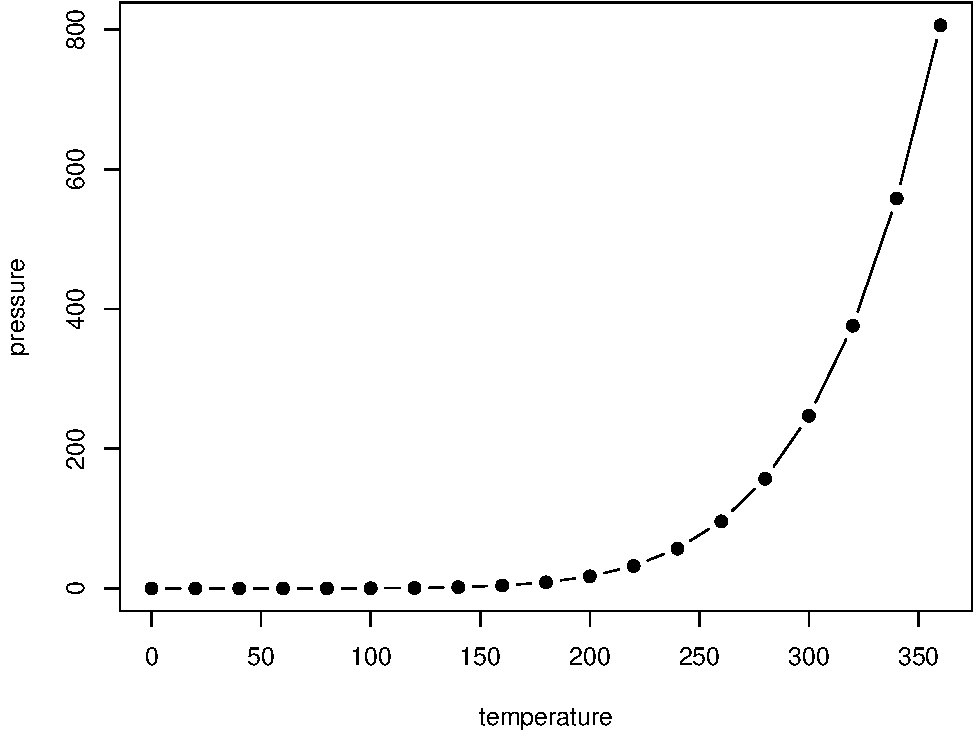
\includegraphics[width=0.8\linewidth]{_main_files/figure-latex/nice-fig-1} 

}

\caption{Here is a nice figure!}\label{fig:nice-fig}
\end{figure}

Don't miss Table \ref{tab:nice-tab}.

\begin{Shaded}
\begin{Highlighting}[]
\NormalTok{knitr}\SpecialCharTok{::}\FunctionTok{kable}\NormalTok{(}
  \FunctionTok{head}\NormalTok{(pressure, }\DecValTok{10}\NormalTok{), }\AttributeTok{caption =} \StringTok{\textquotesingle{}Here is a nice table!\textquotesingle{}}\NormalTok{,}
  \AttributeTok{booktabs =} \ConstantTok{TRUE}
\NormalTok{)}
\end{Highlighting}
\end{Shaded}

\begin{table}

\caption{\label{tab:nice-tab}Here is a nice table!}
\centering
\begin{tabular}[t]{rr}
\toprule
temperature & pressure\\
\midrule
0 & 0.0002\\
20 & 0.0012\\
40 & 0.0060\\
60 & 0.0300\\
80 & 0.0900\\
\addlinespace
100 & 0.2700\\
120 & 0.7500\\
140 & 1.8500\\
160 & 4.2000\\
180 & 8.8000\\
\bottomrule
\end{tabular}
\end{table}

\hypertarget{parts}{%
\chapter{Parts}\label{parts}}

You can add parts to organize one or more book chapters together. Parts can be inserted at the top of an .Rmd file, before the first-level chapter heading in that same file.

Add a numbered part: \texttt{\#\ (PART)\ Act\ one\ \{-\}} (followed by \texttt{\#\ A\ chapter})

Add an unnumbered part: \texttt{\#\ (PART\textbackslash{}*)\ Act\ one\ \{-\}} (followed by \texttt{\#\ A\ chapter})

Add an appendix as a special kind of un-numbered part: \texttt{\#\ (APPENDIX)\ Other\ stuff\ \{-\}} (followed by \texttt{\#\ A\ chapter}). Chapters in an appendix are prepended with letters instead of numbers.

\hypertarget{footnotes-and-citations}{%
\chapter{Footnotes and citations}\label{footnotes-and-citations}}

\hypertarget{footnotes}{%
\section{Footnotes}\label{footnotes}}

Footnotes are put inside the square brackets after a caret \texttt{\^{}{[}{]}}. Like this one \footnote{This is a footnote.}.

\hypertarget{citations}{%
\section{Citations}\label{citations}}

Reference items in your bibliography file(s) using \texttt{@key}.

For example, we are using the \textbf{bookdown} package \citep{R-bookdown} (check out the last code chunk in index.Rmd to see how this citation key was added) in this sample book, which was built on top of R Markdown and \textbf{knitr} \citep{xie2015} (this citation was added manually in an external file book.bib).
Note that the \texttt{.bib} files need to be listed in the index.Rmd with the YAML \texttt{bibliography} key.

The RStudio Visual Markdown Editor can also make it easier to insert citations: \url{https://rstudio.github.io/visual-markdown-editing/\#/citations}

\hypertarget{blocks}{%
\chapter{Blocks}\label{blocks}}

\hypertarget{equations}{%
\section{Equations}\label{equations}}

Here is an equation.

\begin{equation} 
  f\left(k\right) = \binom{n}{k} p^k\left(1-p\right)^{n-k}
  \label{eq:binom}
\end{equation}

You may refer to using \texttt{\textbackslash{}@ref(eq:binom)}, like see Equation \eqref{eq:binom}.

\hypertarget{theorems-and-proofs}{%
\section{Theorems and proofs}\label{theorems-and-proofs}}

Labeled theorems can be referenced in text using \texttt{\textbackslash{}@ref(thm:tri)}, for example, check out this smart theorem \ref{thm:tri}.

\begin{theorem}
\protect\hypertarget{thm:tri}{}\label{thm:tri}For a right triangle, if \(c\) denotes the \emph{length} of the hypotenuse
and \(a\) and \(b\) denote the lengths of the \textbf{other} two sides, we have
\[a^2 + b^2 = c^2\]
\end{theorem}

Read more here \url{https://bookdown.org/yihui/bookdown/markdown-extensions-by-bookdown.html}.

\hypertarget{callout-blocks}{%
\section{Callout blocks}\label{callout-blocks}}

The R Markdown Cookbook provides more help on how to use custom blocks to design your own callouts: \url{https://bookdown.org/yihui/rmarkdown-cookbook/custom-blocks.html}

\hypertarget{sharing-your-book}{%
\chapter{Sharing your book}\label{sharing-your-book}}

\hypertarget{publishing}{%
\section{Publishing}\label{publishing}}

HTML books can be published online, see: \url{https://bookdown.org/yihui/bookdown/publishing.html}

\hypertarget{pages}{%
\section{404 pages}\label{pages}}

By default, users will be directed to a 404 page if they try to access a webpage that cannot be found. If you'd like to customize your 404 page instead of using the default, you may add either a \texttt{\_404.Rmd} or \texttt{\_404.md} file to your project root and use code and/or Markdown syntax.

\hypertarget{metadata-for-sharing}{%
\section{Metadata for sharing}\label{metadata-for-sharing}}

Bookdown HTML books will provide HTML metadata for social sharing on platforms like Twitter, Facebook, and LinkedIn, using information you provide in the \texttt{index.Rmd} YAML. To setup, set the \texttt{url} for your book and the path to your \texttt{cover-image} file. Your book's \texttt{title} and \texttt{description} are also used.

This \texttt{gitbook} uses the same social sharing data across all chapters in your book- all links shared will look the same.

Specify your book's source repository on GitHub using the \texttt{edit} key under the configuration options in the \texttt{\_output.yml} file, which allows users to suggest an edit by linking to a chapter's source file.

Read more about the features of this output format here:

\url{https://pkgs.rstudio.com/bookdown/reference/gitbook.html}

Or use:

\begin{Shaded}
\begin{Highlighting}[]
\NormalTok{?bookdown}\SpecialCharTok{::}\NormalTok{gitbook}
\end{Highlighting}
\end{Shaded}


  \bibliography{book.bib,packages.bib}

\end{document}
